\documentclass[a4paper,12pt]{article} %Dokumendiklassi defineerimine ja väljastatava teksti suuruse seadistamine       
\usepackage{graphicx} %Võimaldab teksti sees kasutada jooniseid
\usepackage[top=2.5cm, bottom=2.5cm, left=3cm, right=3cm]{geometry} %Määrab ära lehekülje suuruse
\usepackage{titlesec} %Vajalik pealkirjade modifitseerimiseks
\usepackage{longtable} %Vajalik pakett, et saaks teha üle ühe leheküljelisi tabeleid
\usepackage{multirow} %Vajalik, kui tahta tabelites mitut rida kokku panna
\usepackage{todonotes} %Vajalik, kui tahta lisada töösse todo märkmeid
\usepackage{url} %Vajalik, kui töös on kasutusel URL aadress. Sel juhul märkida URL tagi vahele ning LaTeX ei hakka seda lahti kompileerima eraldi käskudeks vms
\usepackage[figure,table,page,section]{totalcount} %Jooniste, tabelite, lehtede ja peatükkide arv
\usepackage{float} %Vajalik töös olevate tabelite ja jooniste vormistamiseks
\usepackage{blindtext}
\usepackage{scrextend}
\addtokomafont{labelinglabel}{\sffamily}
\usepackage{longtable} %Korda tabeli päist uuel lehel
\usepackage{color,xcolor,colortbl}% Värvid

\definecolor{codegreen}{rgb}{0,0.6,0}
\definecolor{codegray}{rgb}{0.5,0.5,0.5}
\definecolor{codepurple}{rgb}{0.58,0,0.82}
\definecolor{rowgray}{gray}{0.85}

\definecolor{dkgreen}{rgb}{0,.6,0}
\definecolor{dkblue}{rgb}{0,0,.6}
\definecolor{dkyellow}{cmyk}{0,0,.8,.3}

\usepackage{listings} %Koodi värvimiseks
\usepackage{inconsolata}
\lstset{
    breaklines=true,
    frame=single,
    basicstyle=\ttfamily
  }
\lstnewenvironment{SQL}
  {\lstset{
    breaklines=true,
    language=SQL,
    frame=single,
    framesep=5pt,
    basicstyle=\normalsize,
    %basicstyle=\footnotesize,
    commentstyle=\color{codegreen},
    keywordstyle=\color{blue},
    numberstyle=\tiny\color{codegray},
    stringstyle=\color{codepurple},
    keepspaces=true,                 
    %numbers=left,                    
    %numbersep=2pt,                  
    showspaces=false,                
    showstringspaces=false,
    showtabs=false,                  
    tabsize=2
  }}
  {}
  
\lstnewenvironment{PHP}
  {\lstset{
    breaklines=true,
    language=PHP,
    frame=single,
    framesep=5pt,
    basicstyle=\normalsize,
    %basicstyle=\footnotesize,
    keywordstyle=\color{dkblue},
    stringstyle=\color{dkgreen},
    identifierstyle=\color{black},
    commentstyle=\color{gray},
    emph=[1]{php},
    emphstyle=[1]\color{black},
    emph=[2]{if,and,or,else,return,do,while,new},
    emphstyle=[2]\color{dkblue},
    keepspaces=true,                 
    %numbers=left,                    
    %numbersep=2pt,                  
    showspaces=false,                
    showstringspaces=false,
    showtabs=false,                  
    tabsize=2
  }}
  {}

\usepackage[estonian]{babel} %Eestikeelsete tähtede kasutamise võimalus
\usepackage[T1]{fontenc} %Vajalik vene ja eesti  keelsete tähtede kasutamiseks
\usepackage[utf8]{inputenc} %UTF8 dekodeerimise kasutamine

\addto\captionsestonian{\def\refname{\centerline{Kasutatud kirjandus}}} %Muudab viidete nime kasutatud kirjanduseks ning paigutab lehe keskele
\addto\captionsestonian{\def\listfigurename{\centerline{Jooniste loetelu}}} %Muudab jooniste nimekirja nime jooniste loeteluks ning paigutab selle lehe keskele
\addto\captionsestonian{\def\listtablename{\centerline{Tabelite loetelu}}} %Muudab tabelite nimekirja nime tabelite loeteluks ning paigutab selle lehe keskele
\addto\captionsestonian{\def\contentsname{\centerline{Sisukord}}}
	
\usepackage{tocloft} %Selleks, et modifitseerida sisukorda
\usepackage{amssymb} %Erisümbolid
\renewcommand{\labelitemi}{\tiny$\blacksquare$} %Loetelude ees kuvatakse ruudukesi

\usepackage{caption} %Vajalik tabelite ja jooniste pealkirjastamisel
\captionsetup{labelsep=period} %Lisab tabeli või joonise nime lõppu punkti

\usepackage{verbatimbox} %Koodi kuvamine lehe keskel

\titlelabel{\thetitle.\quad} %Lisab pealkirjade lõppu punkti

\usepackage{times} %Tekst on Times tüüpi
\usepackage{fancyhdr} %Võimaldab kasutada päiseid ja jaluseid
\setlength{\parindent}{0cm} %Lõigu taane on seatud nulliks
\usepackage{setspace} %Vajalik teksti vahede seadistamiseks
\onehalfspacing %Ridade vahel on 1,5 tähe kõrgusest
\setlength{\parskip}{12pt}%Lõiguvahe

\usepackage{hyperref} %Muudab lingid klikitavaks

\hyphenation{} %Ebakorrektse poolitamise parandamine kujul: \hyphenation{üliõpilas-kood lehe-küljed}

\titleformat{\section}{\normalfont\Large\bfseries}{\thesection}{16pt}{} %Sectioni tekstisuurus
\titleformat{\subsection}{\normalfont\large\bfseries}{\thesubsection}{14pt}{} %Subsectioni tekstisuurus
\titleformat{\subsubsection}{\normalfont\normalsize\bfseries}{\thesubsubsection}{12pt}{} %Subsubsectioni tekstisuurus

\titlespacing*{\section}{0pt}{60pt}{18pt} %Sectioni ees, ülal ja all olev ruum
\titlespacing*{\subsection}{0pt}{24pt}{12pt} %Subsectioni  ees, ülal ja all olev ruum
\titlespacing*{\subsubsection}{0pt}{12pt}{12pt} %Subsubsectioni ees, ülal ja all olev ruum

\newcommand{\sectionbreak}{\clearpage} % Iga section algab uuelt lehelt

\begin{document}

%------------------------------TIITELLEHT---------------------------------
\thispagestyle{empty}
\begin{center}
\begin{Large} %Tekst suurtähtedega ja suuremaks
TALLINNA TEHNIKAÜLIKOOL\\
\end{Large}
Infotehnoloogia teaduskond\\
Informaatika instituut
\end{center}

\vspace*{80pt} %Tekitab lehe alguse ja teksti vahele tühja ala vastava laiusega

\begin{center} %Tekst keskele
IDU70LT\\
Rait Raidma 143682\\
\vspace*{40pt}
\begin{LARGE}
POSTGRESQL ANDMEBAASISÜSTEEMI PÕHINE METAANDMETEGA JUHITAVATE VEEBIRAKENDUSTE KIIRPROGRAMMEERIMISE KESKKOND\\
\end{LARGE}
\vspace*{60pt}
Magistritöö
\end{center}
\vspace*{40pt}
\begin{flushright} %Joondab teksti paremale
\begin{tabular}{p{60pt}p{100pt}}
Juhendaja:&Erki Eessaar\\
&Doktor\\
&dotsent\\
\end{tabular}
\end{flushright}
\vspace*{80pt}
\begin{center}
Tallinn 2016
\end{center}
\pagebreak %Lehe lõpp

%---------------------------AUTORIDEKLARATSIOON-------------------------
\section*{\centerline{Autorideklaratsioon}}
Kinnitan, et olen koostanud antud lõputöö iseseisvalt  ning seda ei ole kellegi teise poolt varem kaitsmisele esitatud. Kõik töö koostamisel kasutatud teiste autorite tööd, olulised seisukohad, kirjandusallikatest ja mujalt pärinevad andmed on töös viidatud.\par
Autor: Rait Raidma\par
09.05.2016

\pagebreak

%---------------------------ANNOTATSIOON---------------------------------
\section*{\centerline{Annotatsioon}}
Käesoleva magistritöö eesmärgiks oli disainida ning realiseerida PostgreSQL andmebaasisüsteemi põhine ja veebipõhine kiirprogrammeerimise keskkond, mis võimaldaks luua veebirakendusi. Loodavad rakendused peavad suhtlema andmebaasiga läbi andmebaasiliidese ning rakenduste väljanägemist ning käitumist peab olema võimalik juhtida andmebaasis hoitavate metaandmetega.\par
Töö käigus uuriti, kuidas saab PostgreSQL andmebaasisüsteem suhelda mitme samas serveris asuva PostgreSQL andmebaasiga ning kust saab infot vajalike andmebaasiobjektide kohta. Seejärel kirjeldati loodava süsteemi funktsionaalsus, disainiti selle andmebaas, kasutajaliides ning rakendus.\par
Töö tulemusena valmis süsteemi kirjeldav dokumentatsioon ning sellele vastav süsteem, mille kasutatavuse valideerimiseks realiseeriti ühe rakenduse näidis-kasutusjuhud. Süsteem võimaldab hallata rakendusi, lehti ning neis olevaid regioone, mida antud töö käigus realiseeriti neli erinevat tüüpi: HTML-tekst, navigatsioon, raport ja vorm.\par
Näidisrakendusele pääseb ligi kasutajanimega \textit{kask@ttu.ee} ja parooliga \textit{test} aadressilt \newline \url{http://apex.ttu.ee/pgapex/public/index.php/app/ruumid}. \par
Töö tulemus avaldati MIT litsentsiga ning on avalikult kättesaadav aadressilt \newline \url{https://github.com/raitraidma/pgapex}.
\par
Lõputöö on kirjutatud eesti keeles ning sisaldab teksti 72 leheküljel, \totalsections{} peatükki, \totalfigures{} joonist, \totaltables{} tabelit.
\pagebreak
%-----------------------------ABSTRACT-----------------------------------
\section*{\centerline{Abstract}}
\subsection*{A PostgreSQL-based Rapid Development Environment for the Metadata-driven Web Applications}
The goal of this master thesis is to design and implement a PostgreSQL-based and web-based rapid development environment for the metadata-driven web applications that store data in the same database server. These web applications must communicate with a database through database interface. Applications' look and behaviour must be possible to manipulate by using metadata that is kept in the database.\par

The work investigates how it is possible to connect with multiple PostgreSQL databases in PostgreSQL database management system and where to look for the information about necessary database objects. After that the system functionality, database, user interface, and application design are described.\par

The outcomes of this thesis are documentation that describes the system and implementatsion of the system. For the creation of the system PHP, PostgreSQL, AngularJS, Bootstrap, and Slim Framework were used. The system uses PostgreSQL's \textit{dblink} extension to communicate to external databases. Information about database objects are asked from \textit{information\_schema} and \textit{pg\_catalog}.
\par
The system allows developers to create applications based on external databases and for each application select the authentication method from the set of two methods (no authentication and authentication based on the database function). Application may contain pages that consist of regions.
Four region types were implemented in the system. HTML region allows us to add HTML-formatted text. Navigation region displays menus that can be used to navigate between application's pages or refer to external ones. Report region displays a table based on a view which rows can be divided between pages. Form region allows us to ask information from a user and send it to external database by calling out a function from external database.
\par
Created system is the result of the first development iteration. Only the most important functionality was implemented to ensure the system's primary usability to create real applications. To validate the results, a sample application  was made to show what the system can do.\par
Sample application can be accessed with username \textit{kask@ttu.ee} and password \textit{test} from \newline \url{http://apex.ttu.ee/pgapex/public/index.php/app/ruumid}.
\par
The result of current thesis is available under MIT licecne from \newline \url{https://github.com/raitraidma/pgapex}.
\par
The thesis is in Estonian and contains 72 pages of text, \totalsections{} chapters, \totalfigures{} figures, \totaltables{} tables.
\pagebreak
%---------------------LÜHENDITE JA MÕISTETE SÕNASTIK---------------------
\section*{\centerline{Lühendite ja mõistete sõnastik}}
\begin{labeling}{Metaandmetega juhitav}
\item [ACID] \textit{Atomicity, Consistency, Isolation, Durability}, atomaarsus, konsistentsus, isoleeritus, püsivus. ``Andmebaasihaldurite puhul tehingutöötluse põhikarakteristikud. Atomaarsus tähendab seda, et andmebaasihaldur tagab kas antud tehingu kõigi tegumite või mitte ühegi toimumise. Konsistentsus tähendab, et pärast tehingu lõppu peab andmebaas olema legaalses olekus. Isoleeritus tähendab, et tehing toimub varjatult teiste operatsioonide eest. Püsivus tähendab seda, et kui kasutajat on juba kord teavitatud tehingu edukast toimumisest, siis tehing jääb kehtima ja seda ei saa olematuks muuta'' \cite{Vallaste}
\item [AJAX] \textit{Asynchronous JavaScript And XML}, asünkroonne JavaScript ja XML. ``Interaktiivsete veebirakenduste loomise meetod, kus andmevahetus brauseri ja veebiserveri vahel toimub ilma, et oleks vaja kogu lehte uuesti laadida'' \cite{Vallaste}
\item [CRUD] \textit{Create Read Update Delete}, lühend, mis tähistab andmetega manipuleerimise nelja põhitegevust: loomine, lugemine, muutmine ja kustutamine
\item [CSRF] \textit{Cross-Site Request Forgery}, rünnak, mille puhul käivitatakse veebirakenduses mingi toiming teisest domeenist tulnud päringu korral
\item [CSS] \textit{Cascading Style Sheets}, kaskaadlaadistik. ``Veebilehtede valmistajatele ja kasutajatele mõeldud laadistik. Laadilehed (style sheets) kirjeldavad, kuidas HTML dokumente esitada kuvaril, printeril või kõnesüntesaatorist kostva kõnena'' \cite{Vallaste}
\item [DOM] \textit{Document Object Model}, dokumendiobjektide mudel. ``Eeskiri selle kohta, kuidas objekte (tekst, pildid, pealkirjad, lingid jne) veebilehel esitada. DOM määrab ära, millised atribuudid kuuluvad millise objekti juurde ning kuidas objekte ja atribuute käsitleda'' \cite{Vallaste}
\item [FSF] \textit{Free Software Foundation}, MTÜ, mis propageerib arvuti kasutajate vabadust ja kaitseb vaba tarkvara kasutajate õigusi
\item [HTML] \textit{HyperText Markup Language}, hüpertekst-märgistuskeel. ``Enimlevinud kodeerimissüsteem (tekstivorming) veebidokumentide loomiseks. HTML koodid ehk märgendid määravad ära selle, kuidas veebileht arvutiekraanil välja näeb'' \cite{Vallaste}
\item [Juurutama] \textit{Deploy}, tarkvara või riistvara töölepanekuga seotud protsesside - installeerimine, konfigureerimine, käitamine, testimine - läbimine \cite{Vallaste}
\item [Kiirprogrammeerimine] \textit{Rapid Application Development}, ``arendussüsteem, mis annab programmeerijatele võimaluse kiiresti programme koostada. Üldiselt on RAD-süsteemides rida graafiliste kasutajaliideste loomiseks mõeldud tööriistu, mis oluliselt lühendab taoliste liideste loomisele kuluvat aega'' \cite{Vallaste}
\item [Metaandmed] ``Andmed andmeelementide kohta, sealhulgas nende andmekirjeldused, ning andmed andmete omanduse, pöördusteede, pääsuõiguste ja muutuvuse kohta'' \cite{metaAndmed}
\item [Metaandmetega juhitav] Süsteemi käitumist ja väljanägemist juhitakse andmetega
\item [OSI] \textit{Open Source Initiative}, organisatsioon, mis propageerib avatud lähtekoodiga tarkvara
\item [SQL süstimine] \textit{SQL Injection}, rünnak, mille puhul kasutaja muudab käivitatavat SQL lauset
\item [SQL] \textit{Structured Query Language}, struktureeritud andmebaasikeel andmete käitlemiseks, õiguste jagamiseks ning andmebaasiobjektide haldamiseks
\item [URL] \textit{Uniform Resource Locator}, internatiaadress. Viit arvutivõrgus olevale ressursile. \cite{Vallaste}
\end{labeling}
\pagebreak
%----------------------------SISUKORD----------------------------------
\tableofcontents
\newpage
%----------------------JOONISTE NIMEKIRI-------------------------------
\listoffigures
\pagebreak
%----------------------TABELITE NIMEKIRI---------------------------------
\listoftables
\pagebreak
%-----------------------------SISSEJUHATUS------------------------------- 
\section{Sissejuhatus}
\label{Sissejuhatus} %Võimaldab pealkirjale viidata \ref käsuga
Tänapäeval on arvutisüsteemi toega infosüsteemid väga laialdaselt kasutusel. Tihti aga puudub võimekus kiirelt reageerida muutuvatele info haldamise ning kuvamise vajadustele, kuna pole piisavalt vastavate oskustega inimesi. Seetõttu oleks palju kasu süsteemist, mis ei nõua kasutajalt programmeerimisoskust mitmes erinevas keeles, vaid võimaldaks infosüsteemi info haldamiseks mõeldud veebirakendusi kiiresti ja mugavalt graafilise kasutajaliidese abil täiendada.

\subsection{Taust ja probleem}
Töö idee sai alguse TTÜ-s õpetatavast ainest ``Andmebaasid II'', mille raames tuleb üliõpilastel ühe õpiväljundina luua andmebaas koos seda kasutava rakendusega, kus rakendus suhtleb andmebaasiga läbi andmebaasiliidese. Antud aines võib kasutada andmebaasisüsteeme PostgreSQL \cite{PostgreSQL} ja Oracle \cite{Oracle_DB}. Juhul, kui andmebaas on loodud Oracle andmebaasisüsteemi abil, siis on üliõpilastel rakenduse loomiseks võimalus kasutada metaandmetega juhitavat veebipõhist kiirprogrammeerimise keskkonda Oracle APEX \cite{Oracle_APEX}. PostgreSQL andmabaasisüsteemiga loodud andmebaasi korral tuleb rakendus programmeerida kasutades näiteks PHP-d \cite{PHP}.
See tähendab, et üliõpilane ei saa keskenduda täielikult andmebaasi täiustamisele, vaid peab tegelema ka lisaprogrammeerimisega. Töö tulemusena valmiva süsteemi abil peaks üliõpilastel olema lihtsam luua veebipõhiseid andmebaasirakendusi, mis kasutavad andmebaasisüsteemina PostgreSQL-i. Samas leiab autor, et valmiv süsteem on piisavalt võimekas, et leida rakendust mujalgi.\par

PostgreSQL on avatud lähtekoodiga ja tasuta pakutav andmebaasisüsteem. 2016. aasta maikuu seisuga on see andmebaasisüsteemide populaarsuse indeksis \cite{dbRanking} viiendal kohal. On hea võimalus, et sellel põhineval arendussüsteemil võiks olla lai kasutajaskond. Oracle samalaadse Oracle APEX arenduskeskkonna abil arendajate kogukond ulatub 300000 inimeseni \cite{oracleApexUsers} ning seda kasutatakse mitmesuguse äritarkvara loomiseks.\par

2008. aastal kaitsti magistritöö \cite{pgdb}, mille käigus juba uuriti sellise süsteemi PostgreSQL-i põhjal realiseerimise võimalust ning realiseeriti esialgne prototüüp. Selle töö tulemused näitasid, et taolisel põhimõttel loodud süsteemi loomine PostgreSQL-i põhjal on põhimõtteliselt võimalik. Paraku oli loodud prototüüp suhteliselt algeline, selle lähtekood läks kaduma ning mingit edasist arendust sellega ei toimunud. Seega tuleb pidada õigustatuks selle süsteemi idee uuesti elule äratamist ja süsteemi täiesti uuesti loomist.\par

Autor tutvus 2008. aasta lõputöö dokumendiga, kuid nii käesoleva süsteemi kavandid kui ka realisatsioon on täiesti uus tulemus.\par

Töö valmis 2016. aasta kevadel Tallinna Tehnikaülikoolis.

\subsection{Ülesande püstitus}
Töö eesmärgiks on disainida ning realiseerida PostgreSQL andmebaasisüsteemi põhine, veebipõhine ja metaandmetega juhitav kiirprogrammeerimise keskkond, mille abil saaks luua teisi veebipõhiseid rakendusi. Need rakendused kasutaksid arendussüsteemiga samas serveris olevaid PostgreSQL andmebaase. Loodavates rakendustes peab andmete pärimine, lisamine, muutmine ning kustutamine käima läbi avaliku andmebaasiliidese e virtuaalse andmete kihi. Kogu vajalik info rakenduste kuvamiseks ja käitumise juhtimiseks tuleb hoida loodava süsteemi metaandmete andmebaasis.\par
Loodav süsteem peab toetama PostgreSQL 9.4 ja PHP 5.5.0 ning tuleb välja anda vaba tarkvara litsentsi all, et soodustada süsteemi laialdasemat levikut ning edasist arendamist.

\subsection{Metoodika}
Esiteks tuleb uurida, kas liideste kasutamine andmebaasi poole peal annab süsteemile mingi eelise. Seejärel tuleb selgeks teha, kas ja kuidas saab PostgreSQL andmebaasisüsteem ja selle kaudu tema teenuseid kasutav rakendus suhelda mitme samas serveris asuva PostgreSQL andmebaasiga. Samuti on vaja selgitada, kuidas küsida teistest andmebaasidest infot liideseid moodustavate andmebaasiobjektide kohta. Lisaks uuritakse, milliseid sarnaseid süsteeme on veel olemas ning kuidas need on üles ehitatud. Viimane võimaldab leida nõudeid uuele süsteemile.\par
Süsteemi kavandamiseks ning töös realiseeritava süsteemi alamosa leidmiseks kasutatakse süsteemi tükeldamist allsüsteemideks. Allsüsteemideks jagamine võimaldab ka süsteemi mudeleid paremini struktureerida ja esitada. Süsteemi kavandamine toimub mitmevaateliselt (andmevaade, funktsionaalne vaade) ja mudelipõhiselt. Kontseptuaalseid andmemudeleid kasutati tehnilise lahenduse e tabelite kirjelduste genereerimiseks.\par
Töö tulemusena valmib veebipõhine süsteem, mille abil saab luua veebirakendusi, mis kasutavad andmebaasiga suhtlemiseks andmebaasiliideseid. Töö tulemuse valideerimiseks loodakse näiterakendus, kus realiseeritakse õppejõu poolt ette antud kasutusjuhud, mis sarnanevad üliõpilastöödes esinevatele kasutusjuhtudele.
\subsection{Ülevaade tööst}
Töö alguses antakse ülevaade, mis on andmebaasiliides, kuidas toimub suhtlus väliste andmebaasidega ning kust saab infot andmebaasiobjektide kohta. Lisaks uuritakse milliseid sarnaseid süsteeme on veel olemas. Seejärel tuuakse välja nõudmised, mida süsteem täitma peab ning kirjeldatakse süsteemi ülesehitust. Lõpuks valideeritakse töö tulemust näiterakenduse realiseerimisega ning antakse ülevaade funktsionaalsustest, mida järgnevate iteratsioonide korral teostada võiks.

\section{Teoreetiline taust}
Selles peatükis uuritakse, kas ning miks peaks andmebaasiga suhtlemine käima läbi avaliku andmebaasiliidese, kuidas saab PostgreSQL andmebaasisüsteem suhelda erinevate samas serveris olevate PostgreSQL andmebaasidega, kust saada infot nendes olevate andmebaasiobjektide kohta ning milliseid sarnaseid süsteeme on juba olemas. Lisaks uuritakse, millise litsentsi all tuleks loodav süsteem avalikustada, et kõik soovijad saaksid seda kasutada nii nagu neil vaja.

\subsection{Andmebaasi avalik liides}
\label{andmebaasi_avalik_liides}
Liides on sõltumatute süsteemide vaheline leping, kus on kirjeldatud, millisel viisil saab üks süsteem teisega suhelda.
Andmebaasis saab liideseid kirjeldada kasutades andmebaasiserveris talletatud rutiine (funktsioone ja protseduure), vaateid ning materialiseeritud vaateid e hetktõmmiseid (vt Joonis \ref{fig_andmebaasi_avalik_liides}).
Sellist liidest nimetatakse ka virtuaalseks andmete kihiks \cite[lk 108]{BuildingTheAgileDatabase}. Liidese avalikkus tähendab, et see on nähtav andmebaasi teenuse tarbijatele e rakendustele. Selle vastandiks on privaatne liides, mida moodustavatele elementidele pole rakendustel otse juurdepääsu, kuid mida võivad sisemiselt kasutada avaliku liidese realiseerimiseks mõeldud andmebaasiobjektid \cite{privateInterface}.
\par
PostgreSQL-is saavad arendajad luua andmebaasi avaliku liidese kasutades vaateid, materialiseeritud vaateid ja funktsioone. Loodav arendussüsteem peab võimaldama luua veebirakendusi, mis kasutavad andmebaasi läbi selle avaliku liidese (st ei pöördu otse baastabelite poole). Samuti peab loodav arendussüsteem kasutama ka ise andmebaasiliidest.
\begin{figure}[H]
\centering
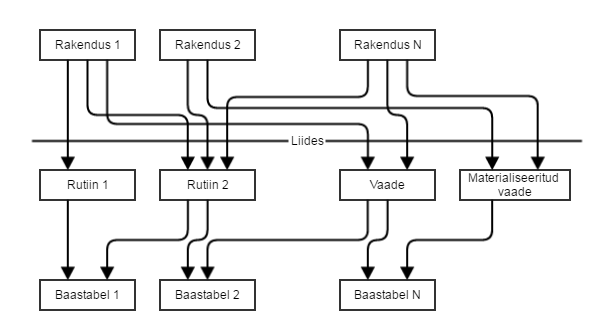
\includegraphics[width=0.8\textwidth]{./diagrams/db-interface.png}
\caption{Andmebaasi avalik liides.}
\label{fig_andmebaasi_avalik_liides}
\end{figure}

\subsubsection{Vaadete kasutamise eelised ja võimalused}
\begin{itemize}
\item Võimaldavad igale rakendusele luua spetsiifilise vaate andmetest, ilma et oleks vaja teha muudatusi andmestruktuurides, mille põhjalt vaateid serveeritakse.
\item Võimaldavad vähendada rakenduse koodi ja andmemudeli vahelist sidusust.
See võimaldab teha muudatusi andmemudelis, ilma, et olemasolev rakendus katki läheks.
\item Neis saab kasutada rakenduse-spetsiifilisi veerunimesid, andmetüüpe ja pikkuseid, mis võimaldab  andmete paremat sidumist rakenduses kasutatavate mudelitega.
\item Võimaldavad ühe täiendava meetme andmete turvalisuse tagamiseks. Kasutajatele või rollidele saab anda õiguse küsida andmeid vaadetest, kuid mitte anda neile õigust lugeda või muuta andmeid baastabelites. Erinevatele kasutajatele saab kuvada andmeid erineval kujul, nii et kasutaja näeb üksnes neid andmeid, mida ta on volitatud nägema. PostgreSQL andmebaasisüsteemis tuleks lisaks kasutada turvabarjääri \textit{WITH (security\_barrier)} lisatingimust. See takistab peidetud ridade kuvamist ka juhul, kui kasutatakse kuritahtlikult valitud funktsioone ja operaatoreid, et näha varjatud infot. \cite{PostgreSQLRulesAndPrivileges}
\item Võimaldavad pärida andmeid erinevatest tabelitest ja andmebaasidest, peites kasutajate eest päringu tegeliku keerukuse. Vaate koostamiseks vajalik päring on eelnevalt koostatud ja optimeeritud. Kui kasutaja teeb vaate, millel on alampäring q1, põhjal päringu q2, siis andmebaasisüsteem koostab q1 ja q2 põhjal uue päringu. Selle täitmiseks kasutatakse vaate aluseks olnud tabelitele loodud indekseid.
\item Võimaldavad varjata rakenduse eest baastabelites olevaid disaini -ja andmevigasid, andes lisaaega nende parandamiseks.
\item Võimaldavad kuvada samu andmeid erineval kujul ühendatuna, kasvõi nt XML või JSON dokumentidena.
\item Läbi vaadete, mis vastavad teatud tingimustele, on võimalik teha andmemuudatusi baastabelites. Lisaks sellele saavad arendajaid vaateid ise andmemuudatusi võimaldavaks ümber programmeerida, kasutades selleks INSTEAD OF trigereid.
\end{itemize}
\cite[lk 172-173]{BuildingTheAgileDatabase}

\subsubsection{Vaadete kasutamisel tekkida võivad probleemid PostgreSQL andmebaasisüsteemi näitel}
Kõik järgnevad punktid osutavad sellele, et tehes vaate põhjal päringu võib andmebaasisüsteem mõnikord koostada täitmisplaani, mille alusel lause täitmine võtab rohkem aega võrreldes sellega, kui päring oleks tehtud otse baastabelite põhjal.
\begin{itemize}
\item Andmebaasisüsteem ei suuda kasutada põhipäringu tingimust (\textit{WHERE} klausel) vaate alampäringus kui vaate alampäringus tehakse ühendi leidmist \textit{UNION} või \textit{UNION ALL} või kui alampäring sisaldab aknafunktsiooni (nt \textit{ROWNUMBER() OVER()} ja \textit{LAG() OVER()})
\item Kui vaate alampäring sisaldab agregaatfunktsiooni (ilma \textit{GROUP BY} klauslita), \textit{ROWNUM} pseudoveergu, aknafunktsiooni \textit{ROWNUMBER() OVER()} või rekursiivset päringut, siis täidetakse vaate põhjal tehtud päring ja vaate alampäring eraldi.
\item Vaate turvabarjääri \textit{WITH (security\_barrier)} kasutamine seab piirangud vaate tingimusklauslite ning vaate põhjal tehtud päringu tingimusklauslite mestimisele.
\item Kui vaate alampäringus viidatakse teistele vaadetele, siis nende vaadete alampäringud täidetakse eraldi.
\end{itemize}
\cite[lk 101-102]{VaadeteMojuParingutele}

\subsubsection{Andmebaasiserveris talletatud rutiinide kasutamise eelised}
\begin{itemize}
\item Üle võrgu saadetavate andmete ja SQL koodi hulk hoitakse minimaalsena, mille tulemusel suureneb rakenduse jõudlus.
\item Rutiinide kood on andmebaasiserveris eelnevalt koostatud ja optimeeritud, suurendades rutiini täitmise efektiivsust.
\item Andmetöötluse jaoks kasutatakse andmebaasiserveri jõudlust, mitte rakendusserveri ega kliendi masina oma.
\item Rutiinis olevat SQL koodi on lihtsam testida ja optimeerida, kui rakendusse sisse kirjutatud SQL-i.
\item Rutiinide käivitusõiguste abil saab piirata andmetele ligipääsu teatud rollidele ning suurendada seeläbi turvalisust.
\item Rutiinis käivitatavad laused tehakse ühe transaktsiooni jooksul. See aitab vältida osalisi andmemuudatusi, kus üks osa muudatustest läheb läbi, teine osa aga mitte.
\end{itemize}
\cite[lk 179, 195]{BuildingTheAgileDatabase}

\subsubsection{Andmebaasiserveris talletatud rutiinide puudused}
\begin{itemize}
\item Koodifunktsionaalsus on piiratud. Rutiinides kasutatavad tsüklid pole nii kiired kui rakenduses. Eriti aeglased ning protsessori-nõudlikud on kursorid.
\item Keerulisemaid rutiine ei pruugi olla võimalik teisaldada ühelt andmebaasisüsteemilt teisele, sest erinevates andmebaasisüsteemides on rutiinide kirjutamiseks kasutusel erinevad keeled.
\item Rutiine on keerulisem grupeerida ning selle tulemusena võib üks ärireegel olla jaotatud mitme rutiini vahele, mis teeb ärireegli haldamise keerulisemaks.
\end{itemize}
\cite{StoredProcProsAndCons}

\subsubsection{Järeldus andmebaasiliideste kasutamise kohta}
Andmebaasiliidesed annavad kasutajale võimaluse vähendada andmebaasi ja rakenduse vahelist sidusust ning suurendada andmete turvalisust ja terviklikust. Mõningatel juhtudel võivad aga vaated ja rutiinid mõjuda operatsioonide jõudlusele nagatiivselt ning rutiinides võib mõningate tegevuste täitmiseks loodava koodi kirjutamine olla keerulisem kui rakenduskihis. Küll aga ei kaalu autori arvates negatiivsed aspektid üle positiivseid, ning seetõttu leiab autor, et andmebaasiliideseid tuleks võimaluse korral siiski kasutada.

\subsection{Ühendumine teiste andmebaasidega}
Kui loodav süsteem installeerida serverisse, kus on mitu andmebaasi, siis  peab kõikide nende andmebaaside põhjal olema võimalik luua rakendusi. Selleks peab loodav süsteem olema võimeline tegema päringuid samas andmebaasiserveris olevatesse teistesse andmebaasidesse (lisaks metaandmete andmebaasile, mida süsteem tööks vajab). PostgreSQL andmebaasisüsteemis ei saa kasutada "tavalisi" andmemuudatuse lauseid, (vt Joonis \ref{fig_sql_andmete_küsimine_välisest_andmebaasist}) mis viitaksid korraga mitmele andmebaasile.
\begin{figure}[H]
\centering
\begin{SQL}
SELECT * FROM other_db_name.schema_name.table_name;
\end{SQL}
\caption{SQL: Andmete küsimine välisest andmebaasist (hüpoteetiline süntaks).}
\label{fig_sql_andmete_küsimine_välisest_andmebaasist}
\end{figure}

Eelnev päring annab tulemuseks veateate (vt Joonis \ref{fig_sql_viga_andmete_küsimisel_välisest_andmebaasist}).
\begin{figure}[H]
\centering
\begin{lstlisting}
ERROR:  cross-database references are not implemented: "other_db_name.schema_name.table_name"
\end{lstlisting}
\caption{SQL viga andmete küsimisel välisest andmebaasist.}
\label{fig_sql_viga_andmete_küsimisel_välisest_andmebaasist}
\end{figure}

Selleks, et ühenduda väliste PostgreSQL andmebaasidega, tuleb kasutada kas \textit{dblink} või \textit{postgres\_fdw} moodulit.

\subsubsection{dblink}
\label{dblink}
Mooduli kasutamiseks tuleb see esmalt installeerida (vt Joonis \ref{fig_sql_dblink_mooduli_installeerimine}).
\begin{figure}[H]
\centering
\begin{SQL}
CREATE EXTENSION IF NOT EXISTS dblink;
\end{SQL}
\caption{SQL: dblink mooduli installeerimine.}
\label{fig_sql_dblink_mooduli_installeerimine}
\end{figure}
Andmete küsimiseks välisest andmebaasist tuleb ette anda andmebaasi nimi, kasutaja ja parool ning lause, mida käivitada soovitakse. Päring käivitatakse välises andmebaasis. Päringuks võib olla iga SQL lause, mis tagastab read (vt Joonis \ref{fig_sql_sql_lause_käivitamine_välises_andmebaasis_dblink_mooduli_abil}). \cite{PostgreSQLdblink}
\begin{figure}[H]
\centering
\begin{SQL}
SELECT schema_name, owner_id
FROM dblink(
  'dbname=external_database_name user=external_database_user password=external_database_user_password',
  'SELECT upper(nspname), nspowner FROM pg_catalog.pg_namespace;'
) AS (
  schema_name varchar,
  owner_id int
);
\end{SQL}
\caption{SQL: SQL lause käivitamine välises andmebaasis dblink mooduli abil.}
\label{fig_sql_sql_lause_käivitamine_välises_andmebaasis_dblink_mooduli_abil}
\end{figure}

\subsubsection{postgres\_fdw}
Selle mooduli poolt pakutav funktsionaalsus kattub suurel määral \textit{dblink} (\ref{dblink}) mooduli funktsionaalsusega, kuid pakub standardsemat süntaksit päringute koostamiseks ning võib \textit{dblink}-i kohati edestada jõudluse poolest.\par
\textit{Postgres\_fdw} loob ühenduse välise serveriga siis, kui tehakse esimene päring välises andmebaasis oleva tabeli vastu. Seda ühendust hoitakse alles ning kasutatakse järgmiste päringute jaoks sama sessiooni piires. Kui väliselt serverilt küsitakse infot erinevate kasutajatena, siis luuakse iga kasutaja jaoks uus ühendus.\par
\textit{Postgres\_fdw} üritab optimeerida väliseid päringuid, et vähendada küsitavate andmete hulka. Selleks saadetakse koos päringuga \textit{WHERE}-klausel ning ei laeta alla veerge, mida pole päringu täitmiseks vaja. Selleks, et vältida valesid päringutulemusi, ei saadeta \textit{WHERE}-klauslit, kui kasutatakse midagi peale sisse ehitatud andmetüüpide, operaatorite ja funktsioonide või kui operaatorid ja funktsioonid pole muutumatud (\textit{immutable}). \cite{PostgreSQLfdw}\par
\textit{Postgres\_fdw} võimaldab lisaks andmete küsimisele (\textit{SELECT}) ka andmeid lisada (\textit{INSERT}), muuta (\textit{UPDATE}) ja kustutada (\textit{DELETE}). Küll aga ei võimalda antud moodul välja kutsuda välises andmebaasis olevaid funktsioone (vt Joonis \ref{fig_sql_funktsiooni_väljakutse}).
\begin{figure}[H]
\centering
\begin{SQL}
SELECT function_from_external_database();
\end{SQL}
\caption{SQL: funktsiooni väljakutse.}
\label{fig_sql_funktsiooni_väljakutse}
\end{figure}

\subsubsection{Mooduli valik}
Kuna loodav süsteem peab suutma välja kutsuda samas serveris asuvates välistes PostgreSQL andmebaasides olevaid funktsioone, siis tuleb kasutada \textit{dblink} (\ref{dblink}) moodulit.

\subsection{Andmebaasiobjektide kirjelduste küsimine}
\label{andmebaasi_objektide_kirjelduste_küsimine}
Loodav süsteem peab teistest andmebaasidest küsima infot andmebaasibjektide kohta, et kuvada süsteemi kasutajale info andmebaasiliidestest, mida rakenduse loomisel on võimalik kasutada. Selleks vajaliku info saab küsida süsteemikataloogidest: \textit{information\_schema} ja \textit{pg\_catalog}.
\textit{Information\_schema} sisaldab vaateid, mis esitavad andmeid andmebaasis olevate andmebaasiobjektide kohta. Kuna \textit{information\_schema} on defineeritud SQL standardis, siis võib eeldada, et selle formaat ei muutu ning seetõttu tuleks eelistada seda kataloogi, et vältida loodava süsteemi katkiminekut  järgmiste PostgreSQL versioonide korral. \cite{PostgreSQLInformationSchema} Küll aga ei sisalda \textit{information\_schema} infot PostgreSQL-spetsiifiliste võimaluste kohta. Selleks tuleb pöörduda \textit{pg\_catalog}-i poole. \textit{Pg\_catalog}-st saab lisaks pärida infot samasse andmebaasiserverisse kuuluvate andmebaaside, materialiseeritud vaadete ning kasutajate paroolide kohta. \cite{PostgreSQLSystemCatalogs} Täpsem loetelu olulisematest süsteemikataloogide vaadetest, mida süsteemi loomisel vaja läheb, on välja toodud Lisas 1.

\subsection{Eksisteerivate programmide analüüs}
Töö käigus uuriti, milliseid sarnaseid süsteeme on veel loodud ning kuidas need on üles ehitatud. Järgnevalt on esitatud lühiülevaade nendest süsteemidest.
\subsubsection{Oracle Application Express (APEX)}
Oracle APEX on veebipõhine rakendus loomaks kiirelt ja lihtsalt teisi veebipõhiseid rakendusi. Kogu süsteem on juhitav andmebaasis hoitavate metaandmetega ning kasutab tööks Oracle andmebaasisüsteemi.\par
APEX (v 5.0.3.00.03) koosneb neljast põhiosast:
\begin{itemize}
\item Application Builder - Võimaldab luua ja hallata uusi rakendusi. Rakendused koosnevad lehtedest. Lehed omakorda sisaldavad regioone. Regioonides võib kuvada raporteid, graafikuid, vorme jpm. Regioonid sisaldavad komponente, mille abil on võimalik kasutajalt infot küsida ning seda esitada. Lisaks on võimalik näha lehtede statistikat ning hallata seadeid.
\item SQL Workshop - Võimaldab näha ja hallata andmebaasiobjekte, käivitada päringuid, importida/exportida andmebaasis olevaid andmeid, koostada päringuid graafilise liidese abil, luua RESTful liideseid jpm.
\item Team Development - Tööde- ja vigadehaldussüsteem. Võimaldab arendajatel ülesandeid planeerida ja hallata.
\item Packaged Apps - Galerii näidisrakendustest, mida on võimalik kohe kasutamiseks installeerida.
\end{itemize}
\cite{Oracle_APEX}
Käesoleva süsteemi idee on tekkinud just Oracle APEX arenduskeskkonna põhjal. Soov on midagi sarnast realiseerida ka PostgreSQL-i jaoks. Käesolevas töös realiseeritav funktsionaalsus on alamosa Oracle APEX-i Application Builderi poolt pakutavast funktsionaalsusest.
\subsubsection{NuBuilder}
NuBuilder on veebipõhine arendusplatvorm loomaks veebipõhiseid rakendusi. Lehtede kirjeldused (sh PHP, JS ja SQL päringud) hoitakse andmebaasis, mis muudab rakenduse varundamise lihtsaks.\par
NuBuilder on kirjutatud PHP-s ning andmeid hoitakse MySQL andmebaasis. Tabelite põhjal on võimalik luua lihtsaid CRUD vorme, kus on võimalik tabelis olevaid andmeid lugeda, lisada, muuta ja kustutada. SQL päringute põhjal on võimalik luua raporteid, mida arendaja saab veebiliidese kaudu disainida. Rakenduse genereerimine toimub PHP-poole peal. \cite{nuBuilder}
Oma kodulehel väidavad nad, et tegu on avatud lähtekoodiga tarkvaraga ning lähtekood on avalikult üleval \cite{nuBuilderGitHub}, kuid kusagil pole mainitud, millise litsentsi alt on tarkvara välja antud. \par
Koodi puhul täheldasin mitut puudujääki:
\begin{itemize}
\item Failid on kehvasti struktureeritud - php, js, png ja gif failid on kõik koos ühes kaustas.
\item PHP ja HTML on kirjutatud läbisegi, mis teeb disaini muutmise keeruliseks.
\item Kasutatakse \$GLOBALS muutujat - see raskendab arusaamist, kus võidakse muutujale programmi töö ajal väärtusi omistada.
\item Funktsioonid on liiga pikad - paljud funktsioonid täidavad korraga liiga palju ülesandeid ja seetõttu on raskendatud nendest arusaamine.
\end{itemize}

\subsubsection{Xataface}
Xataface on programm, millega saab tabelite põhjal genereerida vorme ja kuvasid. Pärast genereerimist tuleb loodud failid serverisse üles laadida. Lehtede konfigureerimine toimub INI failide abil.\cite{Xataface}\par
Xataface on avatud lähtekoodiga ning antud välja GPL litsentsi all. Programm on kirjutatud PHP-s \cite{PHP} ning andmebaasisüsteemina kasutatakse MySQL-i \cite{MySQL}.\par
Kasutatud on palju väliseid teeke. Programmil on üks põhiline arendaja ning igapäevast arendustööd ei toimu. \cite{XatafaceGitHub}
\subsubsection{Andmetega juhitav arendussüsteem PostgreSQL andmebaasirakenduste genereerimiseks}
Tegu on Mati Metsise magistritöö \cite{pgdb} tulemusega. Paraku läks selle lähtekood kaduma ning edasist arendust sellega ei toimunud. Küll aga on olemas dokument, mille põhjal on võimalik saada ülevaade, mida tema poolt loodud prototüüp võimaldas teha.\par
Prototüübis realiseeriti alamosa dokumendis kirjeldatud funktsionaalsusest. Loodud süsteem võimaldas luua rakendusi ja lisada neisse lehti, mis omakorda sisaldasid regioone. Raporti tüüpi regioon genereeriti SQL päringu põhjal. Lisaks oli võimalik luua vorme. Valikkasti ja raadionupu väärtuste määramine käis SQL-päringu abil. Iga rakenduse jaoks loodi andmebaasi uus skeem. Andmete muutmise võimalust antud töös ei realiseeritud.\par
Dokumendi põhjal jäi mulje, et prototüüp ei genereerinud loodud rakendust andmebaasi poolel, vaid seda tehti PHP-abil rakenduskihis.
\subsection{Täpsustunud ülesande püstitus}
Kasutades PostgreSQL 9.4 andmebaasisüsteemi \cite{PostgreSQL} ja PHP 5.5 skriptimiskeelt \cite{PHP}, tuleb realiseerida veebipõhine arendussüsteem, mille abil saab luua teisi veebirakendusi. Tarkvara versioonid, mille põhjal süsteemi arendati, valiti lähtuvalt süsteemi esimese kasutaja käsutuses olevast keskkonnast. Süsteem on vaja luua nii, et see töötaks ka hilisemate versioonide põhjal. Loodavad rakendused peavad andmebaasiga suhtlemiseks kasutama vaadete, materialiseeritud vaadete ja funktsioonide abil loodud andmebaasi avalikku liidest (\ref{andmebaasi_avalik_liides}). Loodav süsteem peab infot liidest moodustavate andmebaasiobjektide kohta küsima samas serveris asuvate väliste PostgreSQL andmebaaside süsteemikataloogidest (\ref{andmebaasi_objektide_kirjelduste_küsimine}) kasutades \textit{dblink} moodulit (\ref{dblink}) ning hoidma seda enda andmebaasis. Kasutamaks võimalikult palju ära andmebaasi võimekust, tuleb rakendused genereerida valmis andmebaasi poole peal. Süsteemi tööpõhimõtet kirjeldab Joonis \ref{fig_süsteemi_tööpõhimõte}. Valminud süsteemi lähtekood tuleb avaldada.

\begin{figure}[H]
\centering
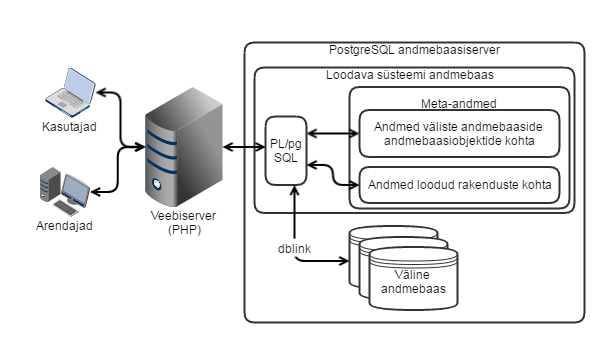
\includegraphics[width=\textwidth]{./diagrams/how-should-pgapex-work.png}
\caption{Süsteemi tööpõhimõte.}
\label{fig_süsteemi_tööpõhimõte}
\end{figure}

\subsection{Litsents}
Üheks töö eesmärgiks oli avaldada loodava prototüübi lähtekood vaba tarkvara litsentsi all. Olemasolevaid litsentse on väga palju. Sobiva litsentsi valimiseks, leian esiteks populaarseimad litsentsid ning võrdlen neid omavahel.
GitHub-i poolt avaldatud statistika kohaselt on 2016. aasta veebruari seisuga populaarseimad litsentsid: MIT (44,69\%), GPLv2 (12,96\%), Apache (11,19\%) ja GPLv3 (8,88\%). \cite{GitHub_Opensource_Licence_Usage}\par
Kõik eelpool nimetatud litsentsid täidavad nii \textit{Free Software} (vt Lisa 2) kui ka \textit{Open Source} (vt Lisa 3) tingimusi. Lisas 4 tabelis \ref{table_litsentside_vordlus} on välja toodud nende litsentside võrdlus.
Loodav süsteem avaldatakse MIT litsentsi all, kuna see seab kasutajatele kõige vähem piiranguid ning arendajale kõige vähem kohustusi.

\section{Süsteemi analüüs}
\label{süsteemi_analüüs}
Järgnevalt leitakse süsteemi tegutsejad ja allsüsteemid ning kirjeldatakse neis realiseeritavad kasutusjuhud.
\subsection{Tegutsejad}
\begin{itemize}
\item Arendaja.
\item Kasutaja.
\end{itemize}
Arendaja on laiendatud õigustega kasutaja, kellele on lubatud hallata süsteemis loodud rakendusi. Kasutaja on arendaja poolt loodud rakenduste lõppkasutaja.
\subsection{Terviksüsteemi tükeldus allsüsteemideks}
Loodav süsteem jagatakse allsüsteemideks, et oleks lihtsam modulaarselt arendada ning struktureeritult kirjeldada loodavat funktsionaalsust.
\subsubsection{Pädevusalad}
\begin{itemize}
\item Arendaja pädevusala.
\item Kasutaja pädevusala.
\end{itemize}
Arendaja pädevusala kasutab kõiki allsüsteeme.\par
Kasutaja pädevusala kasutab ainult rakenduse allsüsteemi.
\subsubsection{Funktsionaalsed allsüsteemid}
\begin{itemize}
\item Rakenduste funktsionaalne allsüsteem.
\item Lehtede funktsionaalne allsüsteem.
\item Regioonide funktsionaalne allsüsteem.
\item Navigatsioonide funktsionaalne allsüsteem.
\item Mallide funktsionaalne allsüsteem.
\end{itemize}
Antud töös ei realiseerita mallide funktsionaalset allsüsteemi, kuna töö maht läheks liiga suureks ning loodav süsteem on kasutatav ka ilma selleta.
\subsubsection{Registrid}
\begin{itemize}
\item Andmebaasiobjektide register. Sellele ei vasta eraldi funktsionaalset allsüsteemi. Sellesse registrisse laaditakse andmeid väliste andmebaaside süsteemikataloogidest. See funktsionaalsus kuulub rakenduste funktsionaalse allsüsteemi alla.
\item Rakenduste register.
\item Lehtede register.
\item Regioonide register.
\item Navigatsioonide register.
\item Mallide register.
\end{itemize}

\subsection{Rakenduste funktsionaalne allsüsteem}
Järgnevalt on esitatud rakenduste funktsionaalse allsüsteemi eesmärgid, kasutatavad registrid ja kasutusjuhtude eskiismudel.
\subsubsection{Eesmärgid}
\begin{itemize}
\item Võimaldada arendajal saada ülevaade loodud rakendustest.
\item Võimaldada värskendada infot andmebaasiobjektide kohta, mille põhjal rakendust luuakse.
\item Võimaldada arendajal luua uus rakendus.
\item Võimaldada arendajal muuta olemasolevate rakenduste seadeid.
\item Võimaldada arendajal kustutada olemasolevaid rakendusi.
\item Võimaldada arendajal muuta rakenduse autentimismeetodit.
\item Võimaldada arendajal ja kasutajal kasutada loodud rakendust.
\end{itemize}
\subsubsection{Allsüsteemi poolt kasutatavad registrid}
Allsüsteem teenindab rakenduste registrit ja andmebaasiobjektide registrit.\par
Allsüsteem kasutab lehtede registrit, regioonide registrit, navigatsioonide registrit ja mallide registrit.
\subsubsection{Allsüsteemi kasutusjuhtude eskiismudel}
Järgnevalt on esitatud rakenduste funktsionaalse allsüsteemi kasutusjuhtude tekstikirjeldused kõrgtaseme formaadis. Kasutusjuhtude mudel on eeskätt tekstiline mudel. Kasutusjuhtude diagramm on sisuliselt selle sisukorraks. Tulenevalt sellest ja tööle seatud mahupiirangutest pidasin paremaks esitada kasutusjuhtude diagrammid siin ja edaspidi lisades. Selle allsüsteemi kasutusjuhtude diagramm on Lisas 5 Joonisel \ref{fig_rakenduste_funktsionaalse_allsüsteemi_kasutusjuhtude_eskiismudel}.

\underline{\textbf{Kasutusjuht:} Kasutaja identifitseerimine}
\par
\textbf{Tegutsejad:} Arendaja
\par
\textbf{Kirjeldus:} Arendaja identifitseerib ennast sisestades kasutajanime ja parooli. Kui sellise kasutajanime ja parooliga kasutaja on andmebaasis olemas ning tal on ülikasutaja õigused, siis lubatakse arendajal süsteemi siseneda, vastasel juhul mitte.
\par
\textit{Märkus:} Kasutusjuht  ``Kasutaja identifitseerimine'' on kasutusel ka järgnevates allsüsteemides: lehtede funktsionaalne allsüsteem, regioonide funktsionaalne allsüsteem, navigatsioonide funktsionaalne allsüsteem.\par

\underline{\textbf{Kasutusjuht:} Andmebaasiobjektide informatsiooni värskendamine}
\par
\textbf{Tegutsejad:} Arendaja
\par
\textbf{Kirjeldus:} Arendaja tahab uuendada infot välistes andmebaasides hoitavate andmebaasiobjektide kohta. Arendajale kuvatakse nupp, millele vajutades uuendatakse infot andmebaasiobjektide kohta ainult nendest andmebaasidest mida loodud rakendused kasutavad.
\par

\underline{\textbf{Kasutusjuht:} Rakenduste loetelu vaatamine}
\par
\textbf{Tegutsejad:} Arendaja
\par
\textbf{Kirjeldus:} Arendaja tahab saada ülevaadet, mis rakendused on loodud. Süsteem kuvab arendajale loetelu rakendustest, kus on esitatud rakenduse nimi. Arendajad näevad kõiki serveris selle vahendi abil loodud rakendusi ja saavad neid kõiki hallata.
\par

\underline{\textbf{Kasutusjuht:} Rakenduse lisamine}
\par
\textbf{Tegutsejad:} Arendaja
\par
\textbf{Kirjeldus:} Arendaja tahab luua uue rakenduse. Arendaja valib rakendusele nime, aliase, andmebaasi, mille põhjal rakendus luuakse ning sisestab andmebaasi kasutajanime ja parooli, kellena süsteem andmebaasiga suhtleb. Kui sisestatud andmed on korrektsed ning sellise kasutajanime ja parooliga kasutaja eksisteerib, siis luuakse uus rakendus. Vigade korral kuvatakse vastavad veateated.
Arendajad saavad rakenduse luua mistahes samas serveris loodud PostgreSQL andmebaasi põhjal, sh ka metaandmete andmebaasi enese põhjal. Kui arendaja soovib andmebaasi põhjal luua uue rakenduse, siis võiks ta andmebaasis luua piiratud õigustega kasutaja, millel on need, ainult need ja täpselt need õigused, mida rakendus vajab andmebaasiga suhtlemiseks. Selle kasutaja kasutajanime ja parooli tuleks kasutada uue rakenduse loomisel.
\par

\underline{\textbf{Kasutusjuht:} Rakenduse muutmine}
\par
\textbf{Tegutsejad:} Arendaja
\par
\textbf{Kirjeldus:} Arendaja valib rakenduse, mida ta soovib muuta. Talle kuvatakse rakenduse nimi, alias, andmebaas, mille põhjal rakendus on loodud ning andmebaasi kasutajanimi. Arendaja saab kuvatud andmeid muuta. Salvestamiseks peab ta sisestama ka andmebaasi kasutajale vastava parooli. Kui sisestatud andmed on korrektsed, siis muudatused salvestatakse. Vigade korral kuvatakse vastavad veateated.
\par

\underline{\textbf{Kasutusjuht:} Rakenduse kustutamine}
\par
\textbf{Tegutsejad:} Arendaja
\par
\textbf{Kirjeldus:} Arendaja valib rakenduse, mida ta soovib kustutada. Enne kustutamist küsitakse temalt kinnitust. Kui arendaja kinnitab kustutamise, siis rakendus ning sellega seotud info kustutatakse.
\par

\underline{\textbf{Kasutusjuht:} Rakenduse autentimismeetodi muutmine}
\par
\textbf{Tegutsejad:} Arendaja
\par
\textbf{Kirjeldus:} Arendaja valib rakenduse, mille autentimismeetodit ta soovib muuta. Talle kuvatakse hetkel kasutusel olev autentimismeetod koos autentimisfunktsiooniga ning sisselogmislehe malliga. Arendaja saab eelpool nimetatud andmeid muuta. Kui sisestatud andmed on korrektsed, siis muudatused salvestatakse. Vigade korral kuvatakse vastavad veateated.
Süsteem peaks välja pakkuma vähemalt kaks autentimismeetodit - autentimine puudub ning autentimine kasutades serveris loodud funktsiooni, millele tuleb ette anda kasutajanimi ja parool ning mis tagastab tõeväärtuse.
\par

\underline{\textbf{Kasutusjuht:} Rakenduse kasutamine}
\par
\textbf{Tegutsejad:} Arendaja, Kasutaja
\par
\textbf{Kirjeldus:} Kasutaja saab kasutada loodud rakendust. Talle kuvatakse aktiivse lehe nähtavate regioonide sisu. Lehel võidakse kuvada navigatsioone, raporteid, vorme ja HTML-teksti. Lehtede vahel saab liikuda klikates navigatsiooniregiooni poolt kuvatavatele linkidele. Kui leht pole valitud, siis suutatakse kasutaja avalehele. Kui rakenduses kuvatav leht nõuab, et kasutaja oleks autenditud, siis kuvatakse kasutajale autentimisvorm, kus küsitakse kasutajanime ja parooli, mille korrektse sisestamise korral lubatakse kasutajal näha kaitstud lehti. Sessiooni jooksul peab autentima ainult ühe korra.
\par

\subsection{Lehtede funktsionaalne allsüsteem}
Järgnevalt on esitatud lehtede funktsionaalse allsüsteemi eesmärgid, kasutatavad registrid ja kasutusjuhtude eskiismudel.
\subsubsection{Eesmärgid}
\begin{itemize}
\item Võimaldada arendajal saada ülevaade rakendusele kuuluvatest lehtedest.
\item Võimaldada arendajal luua uusi lehti.
\item Võimaldada arendajal muuta olemasolevate lehtede seadeid.
\item Võimaldada arendajal kustutada olemasolevaid lehti.
\end{itemize}
\subsubsection{Allsüsteemi poolt kasutatavad registrid}
Allsüsteem teenindab lehtede registrit.\par
Allsüsteem kasutab mallide registrit.
\subsubsection{Allsüsteemi kasutusjuhtude eskiismudel}
Järgnevalt on esitatud lehtede funktsionaalse allsüsteemi kasutusjuhtude tekstikirjeldused kõrgtaseme formaadis. Ruumipuuduse tõttu on kasutusjuhtude ekiismudel esitatud Lisas 5 Joonisel \ref{fig_lehtede_funktsionaalse_allsüsteemi_kasutusjuhtude_eskiismudel}.

\underline{\textbf{Kasutusjuht:} Lehtede loetelu vaatamine}
\par
\textbf{Tegutsejad:} Arendaja
\par
\textbf{Kirjeldus:} Arendaja tahab saada ülevaadet, mis lehed on rakenduse alla loodud. Süsteem kuvab talle loetelu lehtedest, kus tuuakse välja lehe id, alias, pealkiri ja info selle kohta, kas leht on avaleht ning kas leht nõuab kasutaja autentimist.
\par

\underline{\textbf{Kasutusjuht:} Lehe lisamine}
\par
\textbf{Tegutsejad:} Arendaja
\par
\textbf{Kirjeldus:} Arendaja tahab luua rakenduse alla uue lehe. Ta sisestab lehe pealkirja, aliase, valib lehe malli, mida kasutatakse lehe kuvamisel ja valib kas leht on avaleht ning kas leht nõuab autentimist. Kui andmed on korrektsed, siis luuakse uus leht. Vastasel korral kuvatakse vastavad veateated.
\par

\underline{\textbf{Kasutusjuht:} Lehe seadete muutmine}
\par
\textbf{Tegutsejad:} Arendaja
\par
\textbf{Kirjeldus:} Arendaja valib lehtede loetelust lehe, mida ta soovib muuta. Talle kuvatakse lehe pealkiri, alias, mall ja info selle kohta kas tegu on avalehega ning kas leht nõuab kasutaja autentimist. Kuvatud andmeid saab muuta. Kui andmed on korrektsed, siis need salvestatakse. Vastasel korral kuvatakse vastavad veateated.
\par

\underline{\textbf{Kasutusjuht:} Lehe kustutamine}
\par
\textbf{Tegutsejad:} Arendaja
\par
\textbf{Kirjeldus:} Arendaja valib lehtede loetelust lehe, mida ta soovib kustutada. Enne kustutamist küsitakse temalt kinnitust. Kui arendaja kinnitab kustutamise, siis leht ning sellega seotud info kustutatakse.
\par

\subsection{Regioonide funktsionaalne allsüsteem}
Järgnevalt on esitatud regioonide funktsionaalse allsüsteemi eesmärgid, kasutatavad registrid ja kasutusjuhtude eskiismudel.
\subsubsection{Eesmärgid}
\begin{itemize}
\item Võimaldada arendajal saada ülevaade lehel olevatest regioonidest.
\item Võimaldada arendajal luua navigatsiooni tüüpi regioone.
\item Võimaldada arendajal luua HTML tüüpi regioone.
\item Võimaldada arendajal luua raporti tüüpi regioone.
\item Võimaldada arendajal luua vormi tüüpi regioone.
\item Võimaldada arendajal muuta olemasolevaid regioone.
\item Võimaldada arendajal kustutada olemasolevaid regioone.
\end{itemize}
\subsubsection{Allsüsteemi poolt kasutatavad registrid}
Allsüsteem teenindab regioonide registrit.\par
Allsüsteem kasutab mallide registrit, navigatsioonide registrit, andmebaasiobjektide registrit.
\subsubsection{Allsüsteemi kasutusjuhtude eskiismudel}
Järgnevalt on esitatud regioonide funktsionaalse allsüsteemi kasutusjuhtude tekstikirjeldused kõrgtaseme formaadis. Ruumipuuduse tõttu on kasutusjuhtude ekiismudel esitatud Lisas 5 Joonisel \ref{fig_regioonide_funktsionaalse_allsüsteemi_kasutusjuhtude_eskiismudel}.

\underline{\textbf{Kasutusjuht:} Regioonide loetelu vaatamine}
\par
\textbf{Tegutsejad:} Arendaja
\par
\textbf{Kirjeldus:} Arendaja tahab saada ülevaadet, mis regioonid on valitud lehe alla loodud. Talle kuvatakse regioonide loetelu, kus esitatakse regiooni asukoht lehel, regiooni tüüp, järjekorranumber, nimi ning info selle kohta, kas regioon on nähtav või peidetud.
\par

\underline{\textbf{Kasutusjuht:} Regiooni kustutamine}
\par
\textbf{Tegutsejad:} Arendaja
\par
\textbf{Kirjeldus:} Arendaja valib regioonide loetelust regiooni, mida ta soovib kustutada. Enne kustutamist küsitakse temalt kinnitust. Kui arendaja kinnitab kustutamise, siis regioon ning sellega seotud info kustutatakse.

\underline{\textbf{Kasutusjuht:} Regiooni haldamine}
\par
\textbf{Tegutsejad:} Arendaja
\par
\textbf{Kirjeldus:} Regiooni lisamisel või muutmisel kuvatakse arendajale vorm, kus küsitakse regiooni nime, järjekorranumbrit, regiooni malli, mida kasutatakse regiooni kuvamisel ning infot selle kohta, kas regioon on nähtav või peidetud. Regiooni muutmise korral on vormi väljad eelnevalt täidetud. Kui esitatud andmed on korrektsed, siis need salvestatakse. Vastasel korral kuvatakse vastavad veateated.

\underline{\textbf{Kasutusjuht:} HTML regiooni haldamine}
\par
\textbf{Tegutsejad:} Arendaja
\par
\textbf{Kirjeldus:} HTML regiooni lisamisel või muutmisel kuvatakse arendajale vorm, kus lisaks kasutusjuhus ``Regiooni haldamine'' esitatud andmetele küsitakse arendajalt ka teksti, mida regioonis kuvada.

\underline{\textbf{Kasutusjuht:} Navigatsiooni regiooni haldamine}
\par
\textbf{Tegutsejad:} Arendaja
\par
\textbf{Kirjeldus:} Navigatsiooni regiooni lisamisel või muutmisel kuvatakse arendajale vorm, kus lisaks kasutusjuhus ``Regiooni haldamine'' esitatud andmetele küsitakse arendajalt ka navigatsiooni malli, kuvamise tüüpi ja navigatsiooni, mille alusel regioon luuakse ning infot selle kohta, kas regiooni kuvamisel tuleb korrata navigatsioonipunkti malli viimast taset, juhul kui navigatsioonipunkti sügavuse jaoks pole eraldi malli defineeritud.

\underline{\textbf{Kasutusjuht:} Raporti regiooni haldamine}
\par
\textbf{Tegutsejad:} Arendaja
\par
\textbf{Kirjeldus:} Raporti regiooni lisamisel või muutmisel kuvatakse arendajale vorm, kus lisaks kasutusjuhus ``Regiooni haldamine'' esitatud andmetele küsitakse arendajalt ka raporti kuvamisel kasutatavat malli, raporti aluseks olevat vaadet, infot selle kohta, kas raporti päist tuleb kuvada või mitte, mitu rida kuvatakse ühel leheküljel, mis URL-parameetriga antakse edasi hetkel aktiivset lehekülge ning mis veergudest raport koosneb. Pärast vaate valimist saab luua raportile veerge. Raporti veerg võib olla kas valitud vaate veerg või link. Raporti veeru loomisel tuleb sisestada veeru pealkiri, järjekorranumber ning info selle kohta, kas kuvatavas tekstis muudetakse HTML-erimärgid (\&, <, >, ", ') ohutuks või mitte. Lingi korral tuleb lisaks sisestada ka URL ja lingi tekst ning võib lisada lisaatribuute lingi vormindamiseks. Raport peab sisaldama vähemalt ühte veergu.

\underline{\textbf{Kasutusjuht:} Vormi regiooni haldamine}
\par
\textbf{Tegutsejad:} Arendaja
\par
\textbf{Kirjeldus:} Vormi regiooni lisamisel või muutmisel kuvatakse arendajale vorm, kus lisaks kasutusjuhus ``Regiooni haldamine'' esitatud andmetele küsitakse arendajalt ka vormi kuvamisel kasutatavat malli, vormi saatmisnupu malli, saatmisnupul kuvatavat teksti, teadet, mida kuvatakse vormi eduka töötlemise korral, teadet, mida kuvatakse, kui vormi töötlemisel tekib viga, URL, kuhu pärast vormi edukat töötlemist edasi suunatakse, funktsiooni, mille alusel vorm luuakse ning info selle kohta, kas vorm tuleb eelnevalt andmetega täita. Pärast funktsiooni valimist kuvatakse funktsiooni parameetrid ning arendaja peab valima, kuidas neid vormis kuvatakse. Selleks peab ta sisestama vormi välja nime, kirjelduse, järjekorranumbri, valima välja tüübi ja malli. Lisaks saab ta valida, kas väli on kogustuslik või mitte, nähtav või peidetud, sisestada välja vaikimisi väärtuse ja kasutajat abistava teksti. Juhul kui välja tüübiks on element, mille abil on võimalik kuvada mitut valikuvõimalust, siis peab arendaja valima vaate ja veerud, mille põhjal valikud luuakse. Kui on valitud vaade, mille põhjal vorm eeltäidetakse, siis peab arendaja ära kirjeldama päringu tingimused, mille alusel leitakse vaatest õige rida ning määrama, millised vormi väljad infoga täidetakse.

\subsection{Navigatsioonide funktsionaalne allsüsteem}
Järgnevalt on esitatud navigatsioonide funktsionaalse allsüsteemi eesmärgid, kasutatavad registrid ja kasutusjuhtude eskiismudel.
\subsubsection{Eesmärgid}
\begin{itemize}
\item Võimaldada arendajal saada ülevaade rakendusele kuuluvatest navigatsioonidest.
\item Võimaldada arendajal luua uusi navigatsioone.
\item Võimaldada arendajal muuta olemasolevaid navigatsioone.
\item Võimaldada arendajal kustutada olemasolevaid navigatsioone.
\item Võimaldada arendajal lisada olemasoleva navigatsiooni alla navigatsioonipunkte.
\item Võimaldada arendajal muuta olemasolevaid navigatsioonipunkte.
\item Võimaldada arendajal kustutada olemasolevaid navigatsioonipunkte.
\end{itemize}
\subsubsection{Allsüsteemi poolt kasutatavad registrid}
Allsüsteem teenindab navigatsioonide registrit.\par
Allsüsteem kasutab lehtede registrit.
\subsubsection{Allsüsteemi kasutusjuhtude eskiismudel}
Järgnevalt on esitatud navigatsioonide funktsionaalse allsüsteemi kasutusjuhtude tekstikirjeldused kõrgtaseme formaadis. Ruumipuuduse tõttu on kasutusjuhtude ekiismudel esitatud Lisas 5 Joonisel \ref{fig_navigatsioonide_funktsionaalse_allsüsteemi_kasutusjuhtude_eskiismudel}.

\underline{\textbf{Kasutusjuht:} Navigatsioonide loetelu vaatamine}
\par
\textbf{Tegutsejad:} Arendaja
\par
\textbf{Kirjeldus:} Arendaja tahab saada ülevaadet, mis navigatsioonid on valitud rakenduse alla loodud. Arendajale kuvatakse navigatsioonide nimede loetelu.
\par

\underline{\textbf{Kasutusjuht:} Navigatsiooni loomine}
\par
\textbf{Tegutsejad:} Arendaja
\par
\textbf{Kirjeldus:} Arendaja tahab luua uut navigatsiooni. Arendajale kuvatakse vorm, kus küsitakse uue navigatsiooni nime. Kui nimi on korrektne, siis luuakse navigatsioon. Vastasel korral kuvatakse vastvad veateated.
\par

\underline{\textbf{Kasutusjuht:} Navigatsiooni muutmine}
\par
\textbf{Tegutsejad:} Arendaja
\par
\textbf{Kirjeldus:} Arendaja valib navigatsiooni, mida ta soovib muuta. Arendajale kuvatakse navigatsiooni nimi, mida ta saab muuta. Kui nimi on korrektne, siis see salvestatakse. Vastasel korral kuvatakse vastavad veateated.
\par

\underline{\textbf{Kasutusjuht:} Navigatsiooni kustutamine}
\par
\textbf{Tegutsejad:} Arendaja
\par
\textbf{Kirjeldus:} Arendaja valib navigatsioonide loetelust navigatsiooni, mida ta soovib kustutada. Enne kustutamist küsitakse temalt kinnitust. Kui arendaja kinnitab kustutamise, siis navigatsioon ning sellega seotud info kustutatakse. Navigatsiooni ei saa kustutada, kui see on mõne navigatsiooniregiooni poolt kasutusel.
\par

\underline{\textbf{Kasutusjuht:} Navigatsioonipunktide loetelu vaatamine}
\par
\textbf{Tegutsejad:} Arendaja
\par
\textbf{Kirjeldus:} Arendaja tahab saada ülevaadet, millised navigatsioonipunktid on navigatsiooni alla loodud. Arendajale kuvatakse loetelu navigatsioonipunktidest, kus on esitatud navigatsioonipunkti järjekorranumber, nimi ja URL või leht, millele ta viitab. Lisaks on välja toodud, millise navigatsioonipunkti alla ta kuulub.
\par

\underline{\textbf{Kasutusjuht:} Navigatsioonipunkti lisamine}
\par
\textbf{Tegutsejad:} Arendaja
\par
\textbf{Kirjeldus:} Arendaja tahab navigatsiooni alla lisada navigatsioonipunkti. Arendajale kuvatakse vorm, kus küsitakse navigatsioonipunkti nime, järjekorranumbrit, ülem-navigat-sioonipunkti ning URL-i või lehte, millele viidatakse. Kui sisestatud andmed on korrektsed, siis luuakse uus navigatsioonipunkt. Vastasel korral kuvatakse vastavad veateated.
\par

\underline{\textbf{Kasutusjuht:} Navigatsioonipunkti muutmine}
\par
\textbf{Tegutsejad:} Arendaja
\par
\textbf{Kirjeldus:} Arendaja tahab muuta olemasolevat navigatsioonipunkti. Arendajale kuvtakse vorm, kus esitatakse olemasoleva navigatsioonipunkti nimi, järjekorranumber, ülem-navigatsioonipunkt ning URL või leht, millele viidatakse. Arendaja saab muuta eelpool nimetatud andmeid. Kui andmed on korrektsed, siis andmed salvestatakse. Vastasel korral kuvatakse vastavad veateated.
\par

\underline{\textbf{Kasutusjuht:} Navigatsioonipunkti kustutamine}
\par
\textbf{Tegutsejad:} Arendaja
\par
\textbf{Kirjeldus:} Arendaja valib navigatsioonipunktide loetelust navigatsioonipunkti, mida ta soovib kustutada. Enne kustutamist küsitakse arendajalt kinnitust. Kui arendaja kinnitab kustutamise, siis navigatsioonipunkt ning sellega seotud info kustutatakse.
\par

\subsection{Mittefunktsionaalsed nõuded}
Tabelis \ref{mittefunktsionaalsed_nõuded} on välja toodud süsteemile esitatud mittefunktsionaalsed nõuded, mida loodav süsteem peab täitma.
\begin{table}[H]%[!htb]
\begin{center}
\caption{Mittefunktsionaalsed nõuded.}
\label{mittefunktsionaalsed_nõuded}
\begin{tabular}{|p{5cm}|p{10cm}|}
\hline
\rowcolor{rowgray}
Tüüp & Nõude kirjeldus \\ \hline
Serveri tarkvara & Andmete hoidmiseks peab kasutama andmebaasisüsteemi PostgreSQL 9.4 või uuemat. Rakendus tuleb luua kasutades PHP 5.5.0 või uuemat. \\ \hline
Keel & Süsteemi kasutajaliides peab olema ingliskeelne. \\ \hline
Kasutajaliides & Kasutajaliides peab olema veebipõhine ning arvestama erinevate resolutsioonidega. \\ \hline
Toetatud veebibrauserid & 
\begin{itemize}
\item Microsoft Internet Explorer 11 või uuem.
\item Mozilla Firefox 43 või uuem.
\item Google Chrome 49 või uuem.
\end{itemize}
 \\ \hline
Andmebaasioperatsioonide töökiirus & Andmebaasioperatsioonid peavad süsteemil aega võtma alla 5 sekundi. \\ \hline
\end{tabular}
\end{center}
\end{table}

\section{Andmebaas}
Kogu rakenduse genereerimine ning selleks vajaliku info hoidmine toimub andmebaasi poole peal. Järgnevalt on kirjeldatud, kuidas rakenduse genereerimine toimub ning milliseid andmeid ja kuidas selleks talletatakse.

\subsection{Rakenduse genereerimine}
Rakenduse genereerimiseks tuleb  funktsioonile pgapex.f\_app\_query\_page ette anda rakenduse asukoht, rakenduse alias või id, lehe alias või id, päringu meetod (GET või POST), päringu päis (\textit{header}), GET-parameetrid ja POST-parameetrid.\par
Esmalt luuakse ajutised tabelid, kuhu transaktsiooni tööaja jooksul kantakse päringu-spetsiifilised seaded (nt rakenduse id ja lehe id), tagastatava päise info, süsteemi poolt genereeritud teated ning regioonide info.
Võimaldamaks sama andmebaasi sessiooni raames genereerida mitu rakenduse lehte antakse ajutistesse tabelitesse andmete lisamisel kaasa ka transaktsiooni id \textit{txid\_current()}.\par
Seejärel kontrollitakse, kas rakendus ja leht on olemas ning avatakse sessioon.
Sessiooni avamisel kontrollitakse kas kasutaja poolt saadetud päised sisaldavad küpsise infot, kus hoitakse sessiooni id-d. Kui sessiooni id on olemas, siis uuendatakse olemasoleva sessiooni aegumistähtaega. Vastasel korral genereeritakse uus sessiooni id, mis salvestatakse andmebaasi ning luuakse küpsis, mis saadetakse kasutajale tagasi päise parameetri \textit{set-cookie} abil.\par
Kui rakendusele saadeti POST päring, siis kontrollitakse, kas kasutaja tahab autentida või salvestada andmeid vormi regiooni abil. Mõlemal juhul kutsutakse välja välises andmebaasis olev funktsioon. Autentimise korral oodatakse funktsioonilt tõeväärtus (\textit{boolean}) tüüpi väärtust mille põhjal otsustatakse, kas kasutajal on ligipääs lubatud või mitte. Kui autentimisfunktsioon tagastab \textit{TRUE}, siis lisatakse sessiooni märge, et kasutaja on autenditud.\par
Nii GET kui ka POST-meetodi korral kontrollitakse, kas kasutajal on ligipääs antud lehele. Kui ei ole, siis tagastatakse rakenduse seadetes määratud autentimisvorm. Kui kasutajal on õigus lehel viibida, siis käiakse läbi lehega seotud nähtavad regioonid ning genereeritakse meta-info põhjal kasutajale tagastatav leht.\par
Funktsioon pgapex.f\_app\_query\_page tagastab JSON-objekti, mis sisaldab kahte välja \textit{header} ja \textit{body}, mis sisaldavad vastavalt kasutajale saadetavat päist ning kuvatavat sisu.

\subsection{Andmebaasikirjeldus}
Järgnevalt esitatakse loodava süsteemi olemi-suhte diagrammid ja neis esitatud olemitüüpide ning nende atribuutide definitsioonid registrite kaupa. Olemi-suhte diagrammide põhjal genereeritud tabelid on Lisas 6. Kuna süsteemi lähtekood on avaldatud ning andmebaasi tabelite kirjeldus luuakse olemi-suhte diagrammide põhjal, siis kasutatakse olemi-suhte diagrammides inglise keelt.

\subsubsection{Andmebaasiobjektide register}
Joonisel \ref{fig_andmebaasiobjektide_registri_olemi_suhte_diagramm} on esitatud andmebaasiobjektide registri olemi-suhte diagramm. Tabelis \ref{table_er_andmebaasiobjektide_registri_olemitüüpide_definitsioonid} on esitatud registrisse kuuluvate olemitüüpide definitsioonid ning tabelis \ref{table_er_andmebaasiobjektide_registri_olemitüüpide_atribuutide_definitsioonid} nende atribuutide definitsioonid.

\begin{figure}[H]
\centering
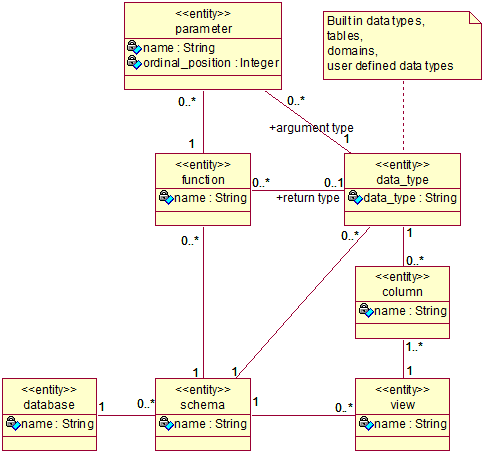
\includegraphics[width=0.9\textwidth]{./diagrams/database-object-er-diagram.png}
\caption{Andmebaasiobjektide registri olemi-suhte diagramm.}
\label{fig_andmebaasiobjektide_registri_olemi_suhte_diagramm}
\end{figure}

\begin{table}[H]
\centering
\caption{Andmebaasiobjektide registri olemitüüpide definitsioonid.}
\label{table_er_andmebaasiobjektide_registri_olemitüüpide_definitsioonid}
\begin{tabular}{|p{4cm}|p{11cm}|}
\hline
\rowcolor{rowgray}
Olemitüübi nimi & Definitsioon \\ \hline
column & Välises andmebaasis olevas vaates esinev veerg\\ \hline
data\_type & Välises andmebaasis kasutusel olev andmetüüp\\ \hline
database & Väline andmebaas on samas serveris asuv PostgreSQL andmebaas, mille kasutamiseks soovitakse rakendust luua. Selleks andmebaasiks võib ka olla metaandmete andmebaas ise\\ \hline
function & Välises andmebaasis olev funktsioon\\ \hline
parameter & Välises andmebaasis oleva funktsiooni parameeter\\ \hline
schema & Välises andmebaasis olev skeem\\ \hline
view & Välises andmebaasis olev vaade\\ \hline
\end{tabular}
\end{table}

\begin{table}[H]
\centering
\caption{Andmebaasiobjektide registri olemitüüpide atribuutide definitsioonid.}
\label{table_er_andmebaasiobjektide_registri_olemitüüpide_atribuutide_definitsioonid}
\begin{tabular}{|p{4cm}|p{4cm}|p{7cm}|}
\hline
\rowcolor{rowgray}
Olemitüübi nimi & Atribuudi nimi & Definitsioon \\ \hline
column & name & Veeru nimi \\ \hline
data\_type & data\_type & Andmetüübi nimi. Selleks võib olla nii andmebaasi sisse ehitatud andmetüüp, domeen või kasuta poolt defineeritud tüüp \\ \hline
database & name & Samas andmebaasiserveris oleva andmebaasi nimi \\ \hline
function & name & Funktsiooni nimi \\ \hline
parameter & name & Parameetri nimi, kui see on olemas \\ \hline
parameter & ordinal\_position & Parameetri esinemisjärjekord funktsioonis \\ \hline
schema & name & Skeemi nimi \\ \hline
view & name & Vaate nimi \\ \hline
\end{tabular}
\end{table}

\subsubsection{Rakenduste register}
Joonisel \ref{fig_rakenduste_registri_olemi_suhte_diagramm} on esitatud rakenduste registri olemi-suhte diagramm. Tabelis \ref{table_er_rakenduste_registri_olemitüüpide_definitsioonid} on esitatud registrisse kuuluvate olemitüüpide definitsioonid ning tabelis \ref{table_er_rakenduste_registri_olemitüüpide_atribuutide_definitsioonid} nende atribuutide definitsioonid.

\begin{figure}[H]
\centering
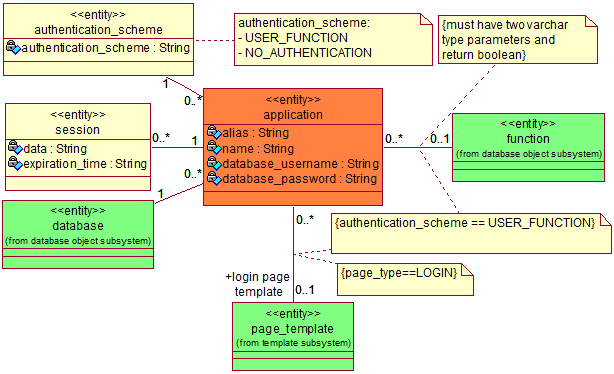
\includegraphics[width=\textwidth]{./diagrams/applications-er-diagram.png}
\caption{Rakenduste registri olemi-suhte diagramm.}
\label{fig_rakenduste_registri_olemi_suhte_diagramm}
\end{figure}

\begin{table}[H]
\centering
\caption{Rakenduste registri olemitüüpide definitsioonid.}
\label{table_er_rakenduste_registri_olemitüüpide_definitsioonid}
\begin{tabular}{|p{4cm}|p{11cm}|}
\hline
\rowcolor{rowgray}
Olemitüübi nimi & Definitsioon \\ \hline
application & Andmebaasi põhjal loodud rakendus \\ \hline
authentication\_scheme & Autentimismeetod, mida kasutatakse autentimist nõudvatel lehtedel \\ \hline
session & Rakenduse kasutaja sessiooniinfo \\ \hline
\end{tabular}
\end{table}

\begin{table}[H]
\centering
\caption{Rakenduste registri olemitüüpide atribuutide definitsioonid.}
\label{table_er_rakenduste_registri_olemitüüpide_atribuutide_definitsioonid}
\begin{tabular}{|p{4cm}|p{4cm}|p{7cm}|}
\hline
\rowcolor{rowgray}
Olemitüübi nimi & Atribuudi nimi & Definitsioon \\ \hline
application & alias & Tähemärkidest ning numbritest koosnev sõne rakenduse tuvastmiseks. Võimaldab luua URL aadressi, kus rakendusele viidatakse aliase abil \\ \hline
application  & name & Rakenduse nimi \\ \hline
application  & database\_username & Kasutaja, kellena süsteem suhtleb välise andmebaasiga \\ \hline
application  & database\_password & Parool, millega sisenetakse välisesse andmebaasi \\ \hline
authentication\_scheme & authentication\_scheme & Autentimismeetod. See võib kas puududa või nõuda funktsiooni, mis teostab õiguste kontrolli \\ \hline
session & data & Rakenduse kasutaja sessioonis hoitavad andmed \\ \hline
session & expiration\_time & Rakenduse kasutaja sessiooni aegumise aeg \\ \hline
\end{tabular}
\end{table}

\subsubsection{Lehtede register}
Joonisel \ref{fig_lehtede_registri_olemi_suhte_diagramm} on esitatud lehtede registri olemi-suhte diagramm. Tabelis \ref{table_er_lehtede_registri_olemitüüpide_definitsioonid} on esitatud registrisse kuuluvate olemitüüpide definitsioonid ning tabelis \ref{table_er_lehtede_registri_olemitüüpide_atribuutide_definitsioonid} nende atribuutide definitsioonid.

\begin{figure}[H]
\centering
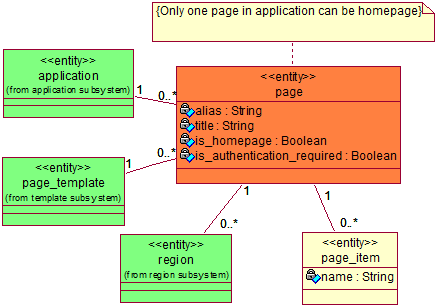
\includegraphics[width=0.8\textwidth]{./diagrams/page-er-diagram.png}
\caption{Lehtede registri olemi-suhte diagramm.}
\label{fig_lehtede_registri_olemi_suhte_diagramm}
\end{figure}

\begin{table}[H]
\centering
\caption{Lehtede registri olemitüüpide definitsioonid.}
\label{table_er_lehtede_registri_olemitüüpide_definitsioonid}
\begin{tabular}{|p{4cm}|p{11cm}|}
\hline
\rowcolor{rowgray}
Olemitüübi nimi & Definitsioon \\ \hline
page & Rakenduses kuvatav leht \\ \hline
page\_item & Lehel kasutatavad vormielemendid ning URL-parameetrid \\ \hline
\end{tabular}
\end{table}

\begin{table}[H]
\centering
\caption{Lehtede registri olemitüüpide atribuutide definitsioonid.}
\label{table_er_lehtede_registri_olemitüüpide_atribuutide_definitsioonid}
\begin{tabular}{|p{3cm}|p{3cm}|p{9cm}|}
\hline
\rowcolor{rowgray}
Olemitüübi nimi & Atribuudi nimi & Definitsioon \\ \hline
page & alias & Tähemärkidest ning numbritest koosnev sõne rakenduses lehe tuvastmiseks. Võimaldab luua URL aadressi, kus lehele viidatakse aliase abil \\ \hline
page & title & Lehel kuvatav pealkiri \\ \hline
page & is\_homepage & Kas tegu on avalehega. Ühel rakendusel saab olla ainult üks avaleht. Kui rakendus sisaldab lehti, siis peab üks leht olema avaleht \\ \hline
page & is\_authentication\newline\_required & Kas lehele pääsemiseks peab kasutaja olema autenditud \\ \hline
page\_item & name  & Vormielemendi või URL-parameetri nimi \\ \hline
\end{tabular}
\end{table}

\subsubsection{Regioonide register}
Joonistel \ref{fig_regioonide_registri_olemi_suhte_diagramm}, \ref{fig_navigatsiooni_regioonide_registri_olemi_suhte_diagramm}, \ref{fig_raportite_regioonide_registri_olemi_suhte_diagramm} ja \ref{fig_vormide_regioonide_registri_olemi_suhte_diagramm} on esitatud regioonide registri olemi-suhte diagramm. Tabelis \ref{table_er_regioonide_registri_olemitüüpide_definitsioonid} on esitatud registrisse kuuluvate olemitüüpide definitsioonid ning tabelis \ref{table_er_regioonide_registri_olemitüüpide_atribuutide_definitsioonid} nende atribuutide definitsioonid.

\begin{figure}[H]
\centering
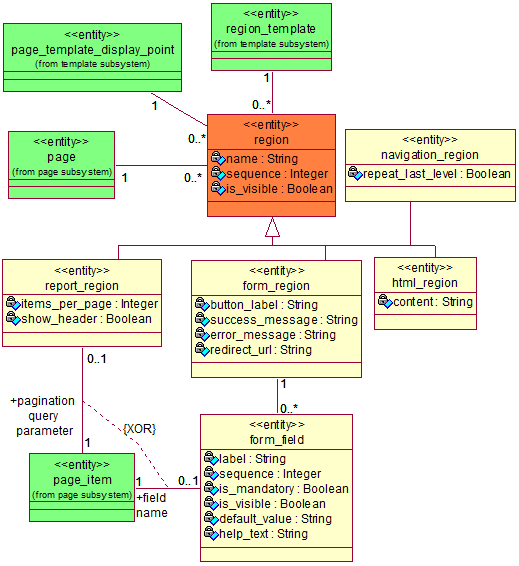
\includegraphics[width=\textwidth]{./diagrams/region-er-diagram.png}
\caption{Regioonide registri olemi-suhte diagramm osa 1.}
\label{fig_regioonide_registri_olemi_suhte_diagramm}
\end{figure}

\begin{figure}[H]
\centering
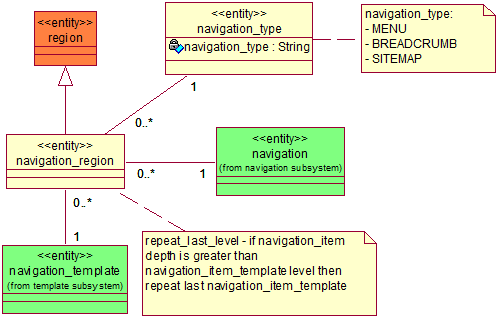
\includegraphics[width=\textwidth]{./diagrams/navigation-region-er-diagram.png}
\caption{Regioonide registri olemi-suhte diagramm osa 2.}
\label{fig_navigatsiooni_regioonide_registri_olemi_suhte_diagramm}
\end{figure}

\begin{figure}[H]
\centering
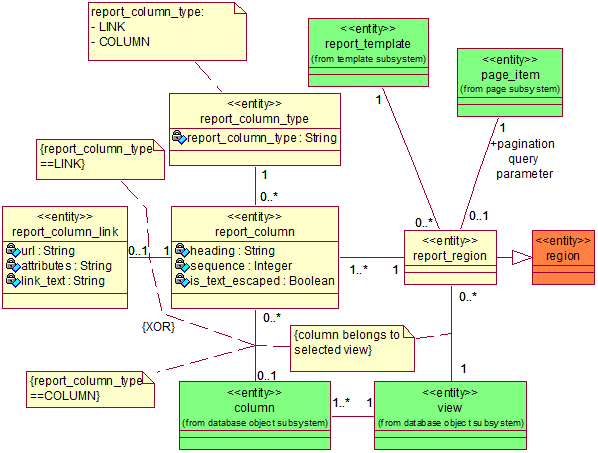
\includegraphics[width=\textwidth]{./diagrams/report-region-er-diagram.png}
\caption{Regioonide registri olemi-suhte diagramm osa 3.}
\label{fig_raportite_regioonide_registri_olemi_suhte_diagramm}
\end{figure}

\begin{figure}[H]
\centering
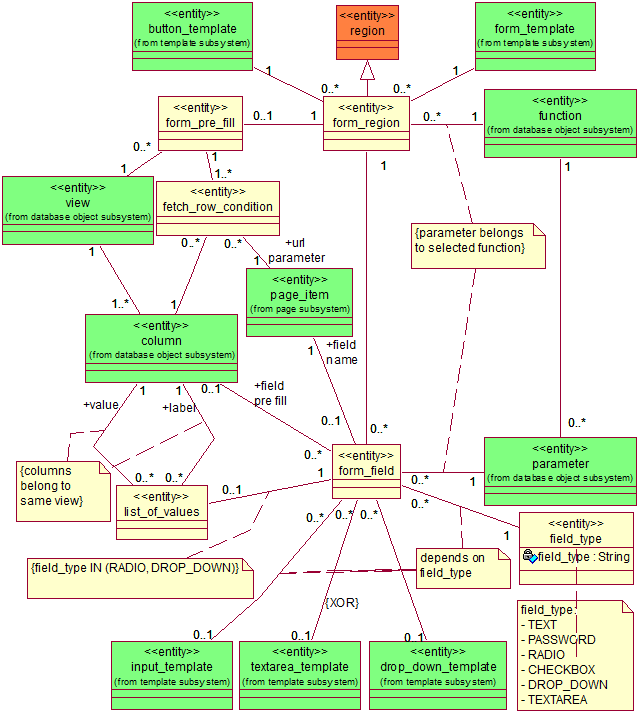
\includegraphics[width=\textwidth]{./diagrams/form-region-er-diagram.png}
\caption{Regioonide registri olemi-suhte diagramm osa 4.}
\label{fig_vormide_regioonide_registri_olemi_suhte_diagramm}
\end{figure}

\begin{table}[H]
\centering
\caption{Regioonide registri olemitüüpide definitsioonid.}
\label{table_er_regioonide_registri_olemitüüpide_definitsioonid}
\begin{tabular}{|p{4cm}|p{11cm}|}
\hline
\rowcolor{rowgray}
Olemitüübi nimi & Definitsioon \\ \hline
fetch\_row\_condition & Tingimus, mille abil küsitakse vaatest rida, mida kasutatakse vormi eeltäitmiseks. Tingimuse kontrolliks vajalik väärtus võetakse URL-parameetrist \\ \hline
field\_type & Vormis kuvatava välja tüüp \\ \hline
form\_field & Vormis kuvatav väli \\ \hline
form\_pre\_fill & Seos vormi eeltäitmiseks vajaliku vaatega \\ \hline
form\_region & Vormi tüüpi regioon \\ \hline
html\_region & HTML tüüpi regioon \\ \hline

\end{tabular}
\end{table}
\begin{table}[H]
\centering
\begin{tabular}{|p{4cm}|p{11cm}|}
\hline
\rowcolor{rowgray}
Olemitüübi nimi & Definitsioon \\ \hline

list\_of\_values & Kui vormi elemendi tüübiks on RADIO või DROP\_DOWN, siis määratakse siin ära, millise vaate väljade põhjal valikud luuakse \\ \hline
navigation\_region & Navigatsiooni tüüpi regioon \\ \hline
navigation\_type & Navigatsiooni tüüp\\ \hline
region & Lehel kuvatav allosa \\ \hline
report\_column & Raportis kuvatav veerg \\ \hline
report\_column\_link & Raportis veerus kuvatav link, kui veeru tüübiks on LINK \\ \hline
report\_column\_type & Raporti veeru tüüp \\ \hline
report\_region & Raporti tüüpi regioon \\ \hline
\end{tabular}
\end{table}

\begin{table}[H]
\centering
\caption{Regioonide registri olemitüüpide atribuutide definitsioonid.}
\label{table_er_regioonide_registri_olemitüüpide_atribuutide_definitsioonid}
\begin{tabular}{|p{3cm}|p{3cm}|p{9cm}|}
\hline
\rowcolor{rowgray}
Olemitüübi nimi & Atribuudi nimi & Definitsioon \\ \hline
field\_type & field\_type & Välja tüübi nimi. Võimalikd väärtused on TEXT, PASSWORD, RADIO, CHECKBOX, DROP\_DOWN, TEXTAREA \\ \hline
form\_field & label & Vormi välja nimi \\ \hline
form\_field & sequence & Vormi välja kuvamise järjekorranumber \\ \hline
form\_field & is\_mandatory & Kas välja täitmine on kohustuslik \\ \hline
form\_field & is\_visible & Kas väli on kasutajale nähtav \\ \hline
form\_field & default\_value & Välja vaikimisi väärtus juhul kui väli on tühi. Võib sisaldada samu muutujaid kui \textit{form\_region.redirect\_url} \\ \hline
form\_field & help\_text & Abistav tekst, mis selgitab, milliseid andmeid kasutajalt oodatakse \\ \hline
form\_region & button\_label & Saatmisnupul kuvatav tekst \\ \hline
form\_region & success\_message & Vormi saatmisel käivitatava välise andmebaasi funktsiooni eduka lõpetamise korral kuvatav tekst \\ \hline
form\_region & error\_message & Vormi saatmisel käivitatava välise andmebaasi funktsiooni ebaeduka lõpetamise korral kuvatav tekst. Lõpetamine loetakse ebaedukaks, kui funktsioon heidab veateate  \\ \hline
form\_region & redirect\_url & Aadress, kuhu kasutaja suunatakse vormi eduka töötlemise korral. Võib sisaldada muutujaid \&APPLICATION\_ROOT\& - rakenduse faili asukoht, \&APPLICATION\_ID\& - rakenduse id, \&PAGE\_ID\& - lehe id, \&USERNAME\& - sisseloginud kasutaja kasutajanimi\\ \hline
html\_region & content & Lehel kuvatav sisu. Võib sisaldada HTML-i \\ \hline
navigation\_region & repeat\_last\_level & Kui navigatsiooni sügavamatele elementidele pole loodud vastavat malli, siis kasutatakse viimast navigatsioonipunkti malli, et kuvada need navigatsioonipunktid. Vastasel juhul jäävad need kuvamata  \\ \hline
navigation\_type & navigation\_type & Navigatsiooni tüüp. Selle põhjal otsustatakse, kuidas tuleb navigatsioon valmis renderdada. Võimalikd väärtused on MENU, BREADCRUMB, SITEMAP \\ \hline

\end{tabular}
\end{table}
\begin{table}[H]
\centering
\begin{tabular}{|p{3cm}|p{3cm}|p{9cm}|}
\hline
\rowcolor{rowgray}
Olemitüübi nimi & Atribuudi nimi & Definitsioon \\ \hline

region & name & Regiooni nimi. Võidakse kuvada lehel \\ \hline
region & sequence & Regiooni kuvamise järjekord \\ \hline
region & is\_visible & Kas regioon on lehel nähtav \\ \hline
report\_column & heading & Raporti veeri päise pealkiri \\ \hline
report\_column & squence & Raporti veeru uvamise järjekord \\ \hline
report\_column & is\_text\_escaped & Kas veerus kuvatavas tekstis muudetakse HTML erimärgid ohutuks \\ \hline
report\_column\newline\_link & url & Aadress, millele link viitab. Võtmesõna \%VEERU\_NIMI\% asendatakse vastavas veerus oleva väärtusega. Võib sisaldada samu muutujaid kui \textit{form\_region.redirect\_url} \\ \hline
report\_column\newline\_link & attributes & Lisaatribuudid, mida on võimalik lingile lisada \\ \hline
report\_column\newline\_link & link\_text & Lingil kuvatav tekst. Võib sisaldada samu võtmesõnu ja muutujaid kui \textit{report\_column\_link.url}\\ \hline
report\_column\newline\_type & report\_column\newline\_type & Raporti veeru tüüp. Võimalikd väärtused on COLUMN, LINK. COLUMN-i korral kuvatakse vaatest saadava välja sisu, LINK-i korral aga link. \\ \hline
report\_region & items\_per\_page & Mitu rida raportist kuvatakse ühel leheküljel. Ülejäänud ridade nägemiseks luuakse lingid \\ \hline
report\_region & show\_header & Kas raportil kuvatakse veerude päiste pealkirjad \\ \hline
\end{tabular}
\end{table}

\subsubsection{Navigatsioonide register}
Joonisel \ref{fig_navigatsioonide_registri_olemi_suhte_diagramm} on esitatud navigatsioonide registri olemi-suhte diagramm. Tabelis \ref{table_er_navigatsioonide_registri_olemitüüpide_definitsioonid} on esitatud registrisse kuuluvate olemitüüpide definitsioonid ning tabelis \ref{table_er_navigatsioonide_registri_olemitüüpide_atribuutide_definitsioonid} nende atribuutide definitsioonid.

\begin{figure}[H]
\centering
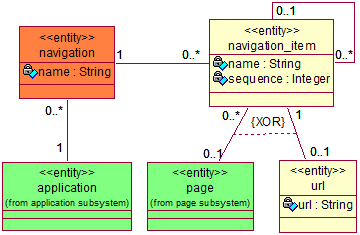
\includegraphics[width=0.7\textwidth]{./diagrams/navigation-er-diagram.png}
\caption{Navigatsioonide registri olemi-suhte diagramm.}
\label{fig_navigatsioonide_registri_olemi_suhte_diagramm}
\end{figure}

\begin{table}[H]
\centering
\caption{Navigatsioonide registri olemitüüpide definitsioonid.}
\label{table_er_navigatsioonide_registri_olemitüüpide_definitsioonid}
\begin{tabular}{|p{4cm}|p{11cm}|}
\hline
\rowcolor{rowgray}
Olemitüübi nimi & Definitsioon \\ \hline
navigation & Navigatsioon grupeerimaks erinevaid navigatsioonihierarhiaid \\ \hline
navigation\_item & Navigatsioonis kuvatav element. Võib sisaldada alamelemente \\ \hline
url & Aadress, kuhu navigatsioonis kuvatav element suunab \\ \hline
\end{tabular}
\end{table}

\begin{table}[H]
\centering
\caption{Navigatsioonide registri olemitüüpide atribuutide definitsioonid.}
\label{table_er_navigatsioonide_registri_olemitüüpide_atribuutide_definitsioonid}
\begin{tabular}{|p{4cm}|p{4cm}|p{7cm}|}
\hline
\rowcolor{rowgray}
Olemitüübi nimi & Atribuudi nimi & Definitsioon \\ \hline
navigation & name & Navigatsiooni kirjeldav nimi \\ \hline
navigation\_item & name & Navigatsioonielemendi kuvamiseks kuvatav tekst \\ \hline
navigation\_item & sequence & Navigatsioonielemendi kuvamisjärjekord oma hierarhia tasemel \\ \hline
url & url & Aadress, kuhu navigatsioonis kuvatav element suunab \\ \hline
\end{tabular}
\end{table}

\subsubsection{Mallide register}
Joonisel \ref{fig_mallide_registri_olemi_suhte_diagramm} on esitatud mallide registri olemi-suhte diagramm. Tabelis \ref{table_er_mallide_registri_olemitüüpide_definitsioonid} on esitatud registrisse kuuluvate olemitüüpide definitsioonid ning tabelis \ref{table_er_mallide_registri_olemitüüpide_atribuutide_definitsioonid} nende atribuutide definitsioonid.

\begin{figure}[H]
\centering
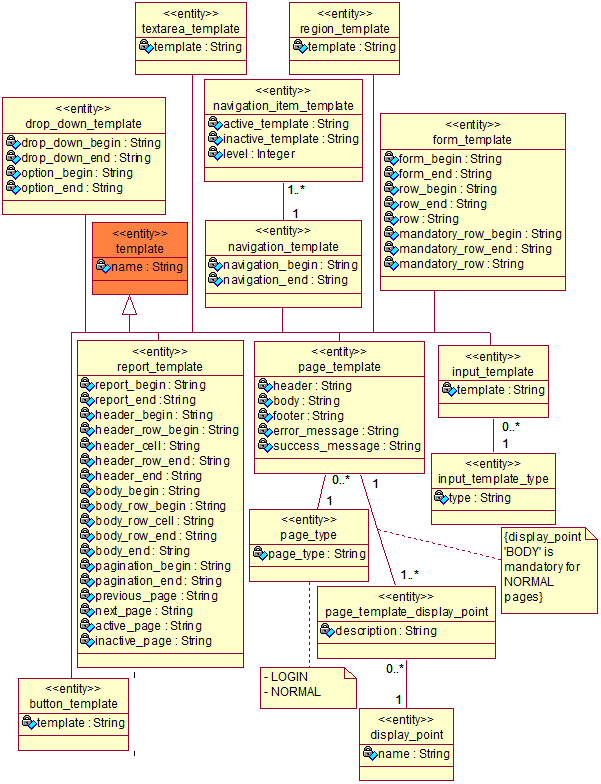
\includegraphics[width=\textwidth]{./diagrams/template-er-diagram.png}
\caption{Mallide registri olemi-suhte diagramm.}
\label{fig_mallide_registri_olemi_suhte_diagramm}
\end{figure}

\begin{table}[H]
\centering
\caption{Mallide registri olemitüüpide definitsioonid.}
\label{table_er_mallide_registri_olemitüüpide_definitsioonid}
\begin{tabular}{|p{5cm}|p{10cm}|}
\hline
\rowcolor{rowgray}
Olemitüübi nimi & Definitsioon \\ \hline
button\_template & Nupu mall \\ \hline
display\_point & Asukohad, kuhu on võimalik lisada regioone \\ \hline
drop\_down\_template & HTML select-elemendi mall \\ \hline
form\_template & Vormi mall \\ \hline
input\_template & HTML input-elemendi mall \\ \hline
input\_template\_type & Võimalikud elemendi kuvamisviisid  \\ \hline
navigation\_item\_template & Navigatsioonipunkti mall \\ \hline
navigation\_template & navigatsiooni mall \\ \hline
page\_template & Lehe mall \\ \hline
page\_template\_display\_point & Lehel kasutatavad asukohad, kuhu on võimalik lisada regioone \\ \hline
page\_type & Lehe malli tüüp \\ \hline
region\_template & Regiooni mall \\ \hline
report\_template & Raporti mall \\ \hline
template & Üldine malli kirjeldus \\ \hline
textarea\_template & HTML textarea-elemendi mall \\ \hline
\end{tabular}
\end{table}

\begin{table}[H]
\centering
\caption{Mallide registri olemitüüpide atribuutide definitsioonid.}
\label{table_er_mallide_registri_olemitüüpide_atribuutide_definitsioonid}
\begin{tabular}{|p{3cm}|p{3cm}|p{9cm}|}
\hline
\rowcolor{rowgray}
Olemitüübi nimi & Atribuudi nimi & Definitsioon \\ \hline
button\_template & template & Nupu mall. Võib sisaldada võtmesõnu \#NAME\# ja \#LABEL\#, mis asendatakse vastavalt vormi elemendi nimega ning kasutajale kuvatava tekstga  \\ \hline
display\_point & name & Asukoha nimi \\ \hline
drop\_down\newline\_template & drop\_down\_begin & HTML select-elemendi algus. Võib sisaldada võtmesõnu \#ROW\_LABEL\# ja \#NAME\#, mis asendatakse vastavalt vormi välja nimega ning vrmi elemendi nimega \\ \hline
drop\_down\newline\_template & drop\_down\_end & HTML select-elemendi lõpp \\ \hline
drop\_down\newline\_template & option\_begin & HTML option-elemendi algus. Võib sisaldada võtmesõnu \#VALUE\# ja \#SELECTED\#, mis asendatakse vastavalt valiku väärtusega ning millega tähistatakse aktiivset valikut\\ \hline
drop\_down\newline\_template & option\_end & HTML option-elemendi lõpp \\ \hline
form\_template & form\_begin & Vormi algus. Võib sisaldada võtmesõna \#SUBMIT\_BUTTON\#, mis asendatakse saatmisnupuga \\ \hline
form\_template & form\_end & Vormi lõpp. Võib sisaldada võtmesõna \#SUBMIT\_BUTTON\#, mis asendatakse saatmisnupuga \\ \hline
form\_template & row\_begin & Vormi rea algus \\ \hline
form\_template & row\_end & Vormi rea lõpp \\ \hline
\end{tabular}
\end{table}

\begin{table}[H]
\centering
\begin{tabular}{|p{3cm}|p{3cm}|p{9cm}|}
\hline
\rowcolor{rowgray}
Olemitüübi nimi & Atribuudi nimi & Definitsioon \\ \hline
form\_template & row & Vormi rida. Võib sisaldada võtmesõnu \#FORM\_ELEMENT\#, \#HELP\_TEXT\# ja \#LABEL\#, mis asendatakse vastavalt vormi elemendi, abistava teksti ja välja nimega \\ \hline
form\_template & mandatory\_row\newline\_begin & Vormi rea algus, mis sisaldab kohustuslikku elementi \\ \hline
form\_template & mandatory\_row\newline\_end & Vormi rea lõpp, mis sisaldab kohustuslikku elementi \\ \hline
form\_template & mandatory\_row & Vormi rida, mis sisaldab kohustuslikku elementi. Võib sisaldada samu võtmesõnu kui \textit{form\_template.row} \\ \hline
input\_template & template & HTML input-elemendi kujundus \\ \hline
input\_template\newline\_type & type & Võimalikud elemendi kuvamisviisid: TEXT, PASSWORD, CHECKBOX, RADIO \\ \hline
navigation\_item\newline\_template & active\_template & Aktiivse navigatsioonielemendi mall \\ \hline
navigation\_item\newline\_template & inactive\_template & Mitteaktiivse navigatsioonielemendi mall \\ \hline
navigation\_item\newline\_template & level & Navigatsioonielemendi sügavus, millal antud malli rakendatakse \\ \hline
navigation\newline\_template & navigation\_begin & Navigatsiooni algus \\ \hline
navigation\newline\_template & navigation\_end & Navigatsiooni lõpp \\ \hline
page\_template & header & Lehe päis. Võib sisaldada võtmesõnu \#TITLE\#, \#APPLICATION\_NAME\#, \#ERROR\_MESSAGE\#, \#SUCCESS\_MESSAGE\#, \#LOGOUT\_LINK\#, mis asendatakse vastavalt lehe pealkirjaga, rakenduse nimega, veateatega, teatega, väljalogimise URL-aadressiga \\ \hline
page\_template & body & Lehe sisuosa. Võib sisaldada samu võtmesõnu kui \textit{page\_template.header} ning lisaks  \#BODY\#, mis asendatakse regiooniga. Võib sisaldada veel teisigi positsiooni määravaid võtmesõnu, mis regioonidega asendatakse \\ \hline
page\_template & footer & Lehe jalus. Võib sisaldada samu võtmesõnu kui \textit{page\_template.header} \\ \hline
page\_template & error\_message & Lehel kuvatav veateade. Võib sisaldada võtmesõna \#MESSAGE\#, mis asendatakse vastava teatega \\ \hline
page\_template & success\_message & Lehel kuvatav teade. Võib sisaldada võtmesõna \#MESSAGE\#, mis asendatakse vastava teatega \\ \hline
page\_template\newline\_display\_point & description & Lehel oleva asukoha kirjeldus \\ \hline
page\_type & page\_type & Lehe malli tüüp. Võimalikud väärtused: LOGIN, NORMAL. NORMAL tüüpi leht peab sisaldama \#BODY\# võtmesõna \\ \hline
region\_template & template & Regiooni mall \\ \hline

\end{tabular}
\end{table}

\begin{table}[H]
\centering
\begin{tabular}{|p{3cm}|p{3cm}|p{9cm}|}
\hline
\rowcolor{rowgray}
Olemitüübi nimi & Atribuudi nimi & Definitsioon \\ \hline

report\_template & report\_begin & Raporti algus. Võib sisaldada võtmesõna \#PAGINATION\#, mis asendatakse lehtedele jaotamise linkidega \\ \hline
report\_template & report\_end & Raporti lõpp. Võib sisaldada samu võtmesõnu kui \textit{report\_template.report\_begin} \\ \hline
report\_template & header\_begin & Raporti päise algus. Võib sisaldada samu võtmesõnu kui \textit{report\_template.report\_begin} \\ \hline
report\_template & header\_row\_begin & Raporti päise rea algus \\ \hline
report\_template & header\_cell & Raporti päise kast, kus kuvatakse veeru pealkiri \\ \hline
report\_template & header\_row\_end & Raporti päise rea lõpp \\ \hline
report\_template & header\_end & Raporti päise lõpp. Võib sisaldada samu võtmesõnu kui \textit{report\_template.report\_begin} \\ \hline
report\_template & body\_begin & Raporti sisuosa algus. Võib sisaldada samu võtmesõnu kui \textit{report\_template.report\_begin} \\ \hline
report\_template & body\_row\_begin & Raporti sisuosa rea algus \\ \hline
report\_template & body\_row\_cell & Raporti sisuosa kast, kus kuvatakse infot \\ \hline
report\_template & body\_row\_end & Raporti sisuosa rea lõpp \\ \hline
report\_template & body\_end & Raporti sisuosa lõpp. Võib sisaldada samu võtmesõnu kui \textit{report\_template.report\_begin} \\ \hline
report\_template & pagination\_begin & Lehtedele jaotamise algus \\ \hline
report\_template & pagination\_end & Lehtedele jaotamise lõpp \\ \hline
report\_template & previous\_page & Link eelmisele lehele. Võib sisaldada võtmesõna \#LINK\#, mis asendatakse viitega eelmisele lehele \\ \hline
report\_template & next\_page & Link järgmisele lehele. Võib sisaldada võtmesõna \#LINK\#, mis asendatakse viitega järgmisele lehele \\ \hline
report\_template & active\_page & Aktiivse lehe link. Võib sisaldada võtmesõnu \#LINK\# ja \#NUMBER\#, mis asendatakse vastavalt lehe aadressiga ning lehe numbriga \\ \hline
report\_template & inactive\_page & Mitteaktiivse lehe link. Võib sisaldada samu võtmesõnu kui \textit{report\_template.active\_page} \\ \hline
template & name & Malli nimi \\ \hline
textarea\_template & template & HTML textarea-elemendi mall \\ \hline
\end{tabular}
\end{table}

\section{Kasutatavad tehnoloogiad ja arendusprotsess}
Järgnevalt antakse ülevaade, miks ja milliseid programme ning raamistikke süsteemi loomisel kasutati. Seejärel antakse ülevaade süsteemi arendamise protsessist.
\subsection{Vagrant}
Vagrant on käsureaprogramm, millega saab hallata virtuaalmasina elutsüklit. Vagrant isoleerib programmilised sõltuvused ja nende konfiguratsioonid ühtsesse eraldiseisvasse keskkonda. Keskkonna konfigureerimiseks saab kasutada käsurea käsklusi, \textit{Ansible}-t \cite{Ansible}, \textit{Puppet}-it \cite{Puppet}, \textit{Chef}-i \cite{Chef}, \textit{Docker}-it \cite{Docker} ja \textit{Salt}-i \cite{Salt}. Tänu Vagrantile saavad kõik luua endale täpselt ühesuguse keskkonna, kus programme käivitada, vähendades võimalust, et ühes arvutis programm töötab, teises aga mitte. \cite{Why_Vagrant}
\subsection{Bower}
Bower on paketihaldussüsteem (\textit{package manager}), mis on mõeldud veebis kasutatavate failide - HTML, CSS, javascript, fondid ja pildid - haldamiseks. Bower-i kasutamiseks peab masinasse olema installitud node, npm ja git. Paketide haldus toimub bower.json failis, kus kirjeldatakse ära soovitud paketid ning nende versioonid. Tänu sellele ei pea arendaja tegelema koodus kasutatavate pakettide haldamisega. \cite{Bower}
\subsection{AngularJS}
Angular on raamistik loomaks dünaamilisi veebirakendusi. See võimaldab laiendada HTML süntaksit, et panna elemendid käituma vastavalt arendaja soovile. Angular kasutab kahe suunalist andmesidumist (\textit{data binding}). See tähendab et muudatused javascripti koodis kajastuvad automaatselt HTML-is ning vastupidi. Tänu sellele peab arendaja vähem tegelema DOM-i manipuleerimisega.  \cite{AngularJS}.
\subsection{Bootstrap}
Bootstrap on mobiilisõbralik kasutajaliidese raamistik, mille abil saab luua dünaamilist veebidisaini (\textit{responsive web design}), mis arvestab kasutaja ekraani suurusega ning kohandab end jooksvalt vastavalt sellele. Bootstrap-is on realiseeritud mitmed komponendid, mis kiirendavad kasutajaliidese loomist. Bootstrap kasutab HTML-i, javascripti js CSS-i. \cite{Bootstrap}
\subsection{TravisCI}
TravisCI on pideva integratsiooni (\textit{continuous integration}) arendusvahend, mille abil saab luua virtuaalse keskkonna koodi kompilleerimiseks, testimiseks ja juurutamiseks. Keskkonna seadistamine toimub faili .travis.yml abil, kus määratakse ära virtuaalkeskkonna operatsioonisüsteem, installitavad teegid ning käivitatavad käsud. \cite{TravisCI}
\subsection{PHP}
PHP \textit{(PHP: Hypertext Preprocessor)} on avatud lähtekoodiga skriptimiskeel, mis on peamiselt mõeldud veebiprogrammeerimiseks. \cite{What_Is_PHP} PHP koodi protsessitakse PHP interpretaatori abil. Üldjuhul kasutatakse interpreteerimiseks \textit{Zend Engine}-t, kuid PHP koodi on võimalik interpreteerida ka \textit{HHVM}-i \cite{HHVM} abil. PHP toetab erinevaid operatsioonisüsteeme, sealhulgas Windows-i erinevaid versioone ja Linuxi erinevaid distributsioone.
\subsection{Composer}
Composer on PHP-s kirjutatud sõltuvuste haldamise süsteem. Sõltuvused kirjeldatakse composer.json failis ning Composer ise tegeleb nende allalaadimisega ning uuendamisega. \cite{Composer}
\subsection{Slim Framework 3}
Slim \cite{SlimFW} on PHP mikro-raamistik. See tähendab, et temas on realiseeritud põhifunktsionaalsused ning paljud lisad on välja jäetud. Kuna loodud süsteemi PHP-rakenduse poolne osa on üpriski õhuke ning lihtne, siis valitigi antud raamistik.\par
Slim koosneb järgmistest põhiosadest:
\begin{itemize}
\item Marsruuter (\textit{router}) analüüsib kasutaja poolt tehtud päringut ning võrdleb seda defineeritud masrtuutidega. Kui marsruutide seast leitakse sobiv vaste, siis initsialiseeritakse vastav kontroller ning päring edastatakse kontrollerile.
\item Kontrollerile (\textit{controller}) antakse ette päringu (\textit{request}) ja vastuse (\textit{response}) objektid. Päringu objekt sisaldab kasutaja poolt saadetud infot ning vastuse objekti peab kontroller lisama kasutajale kuvatava vastuse.
\item Vahevara (\textit{middleware}) abil on võimalik manipuleerida päringu ja vastuse objekte enne ning pärast kontrollerisse jõudmist.
\end{itemize}

\subsection{Postgresql}
PostgreSQL on avatud lähtekoodiga objekt-relatsiooniline andmebaasisüsteem, mis vastab täielikult \textit{ACID} nõuetele. See toetab muuhulgas välisvõtmete deklareerimist, tabelite ühendamise operatsioone, vaateid, trigereid ja andmebaasiserveris talletatud funktsioone. PostgreSQL toetab erinevaid operatsioonisüsteeme, sealhulgas Windows-i erinevaid versioone ja Linuxi erinevaid distributsioone.
\cite{PostgreSQL_About}
\subsection{Arendusprotsess}
Sellise mahuka ja potentsiaalselt väga suure funktsionaalsuse hulgaga süsteemi puhul on selge, et arendus peab toimuma iteratiivselt ja inkrementaalselt ning magistritöö tulemusena pole reaalne tervet süsteemi valmis saada. \par

Alustuseks sai paika pandud esmased nõuded, mida süsteem peaks võimaldama teha. Kuna süsteemi esimene võimalik kasutuskoht oleks TTÜ-s õpetatavas aines ``Andmebaasid II'', siis konsulteeriti antud õppeaine õppejõuga ning kaardistati enamlevinud kasutusjuhud, mida antud aine raames tuleb üliõpilastel andmebaasirakenduste ehitamisel realiseerida.

Neid silmas pidades loodi süsteemi esialgne tükeldus allsüsteemideks, mida koos juhendajaga üle vaadates pandi paika prioriteedid ja määrati kindlaks allsüsteemid, millele antud töös keskenduda. Need allsüsteemid on toodud välja ka töö peatükis \ref{süsteemi_analüüs}.
\par


Allsüsteemide tükeldust silmas pidades loodi süsteemi kasutatavaid metaandmeid kirjeldav kontseptuaalne andmemudel ning kasutajaliidese prototüüp, mis võeti hiljem loodavas süsteemis kasutusele. 
Prototüüp kasutas andmete kuvamiseks võltsandmeid. See andis hea ettekujutuse loodava süsteemi võimekusest ning aitas juhtida tähelepanu aspektidele, millele ilma prototüübi abita ei oleks kohe tuldud. Kontseptuaalsele andmemudelile teisendusreegleid rakendades jõuti metaandmete andmebaasi tabelite kirjeldusteni.\par

Selleks, et loodavat süsteemi oleks ka teistel arendajatel lihtsam kasutusele võtta ning täiustada, sai arenduskeskkonna loomiseks kasutatud Vagrant-i \cite{Vagrant}, mille abil loodi virtuaalmasin koos kõigi arenduseks vajalike teekidega. Virtuaalmasina konfigureerimiseks kasutati bash-i skripti.\par

Dünaamilise kasutajaliidese loomiseks kasutati AngularJS 1.4 \cite{AngularJS}. Lihtsustamaks kasutajaliidese ühtset väljanägemist erinevates veebilehitsejates ning eri suurustes ekraanidega, kasutati Bootstrap 3 \cite{Bootstrap}. Kasutajaliidese poolt kasutatavaid sõltuvusi hallati Bower-i \cite{Bower} abil. Koodi kvaliteedi kontrollimiseks ja säilitamiseks kirjutati testid, mille käivitamiseks kasutati Karma-t \cite{Karma}.\par

Arendussüsteemi andmebaasi loomisel lähtuti ideest, et kogu suhtlus andmebaasiga peab käima läbi andmebaasiliidese (\ref{andmebaasi_avalik_liides}). Andmete salvestamiseks ning küsimiseks tuleb kasutajal välja kutsuda vastav andmebaasifunktsioon. Kasutamaks ära PostgreSQL-i \cite{PostgreSQL} võimalust väljastada JSON tüüpi andmeid, luuakse kasutajaliidese jaoks vajalik vastus juba andmebaasis. Tänu sellele pole andmetega manipuleerimine süsteemis laiali jaotatud vaid toimub üksnes andmebaasi poolel.\par

Andmebaasi ja kasutajaliidese vaheline suhtlus toimub läbi PHP-s \cite{PHP} kirjutatud rakenduse. Kuna antud rakenduse kiht on üpriski õhuke, siis sai selle loomiseks valitud ka lihtsakoeline raamistik Slim Framework 3 \cite{SlimFW}. PHP-s kirjutatud koodi testimiseks kasutati PHPUnit-it \cite{PHPUnit} ning Mockery-t \cite{Mockery}. Koodi sõltuvusi hallati Composer-i abil \cite{Composer}. \par

Koodi hoidmiseks kasutatakse GitHub-i \cite{GitHub}. Iga kord, kui koodihoidlasse midagi üles laetakse luuakse TravisCI-s \cite{TravisCI} virtuaalkeskkond, kuhu tõmmatakse GitHub-st loodava süsteemi kood ning testide eduka läbimise korral juurutatakse serverisse. Tänu sellele on serveris alati näha süsteemi viimane töötav version.

\section{Kasutajaliides}
Kasutajaliides koosneb neljast põhiosast, milleks on moodulid, vaated, teenused ning tõlkefailid. Iga allsüsteemi haldamiseks ning kasutajate autentimiseks on loodud eraldi moodul. Moodulis on ära määratud, mis lehe korral mingi kontroller käivitatakse ning millist vaadet kasutatakse. Vaadete osas on ära kirjeldatud erinevate lehtede väljanägemine ning teenuste osas suhtlus. Kuigi hetkel ei ole arendajatel võimalus kasutajaliidese keelt muuta, tuleb kogu kuvatav tekst tõlkefailidest. Seetõttu on lihtne tõlkida süsteemi ka teistesse keeltesse.\par
Lehele minnes kontrollitakse, mis URL-ile kasutaja tuli ja käivitatakse vastav kontroller ning laetakse sisse vaade, mida antud kontroller kasutab. Kontrolleri käivitamisel antakse talle ette tööks vajalikud teenuste objektid. Selleks kasutatakse sõltuvuste süstimise disainimustrit. See tähendab, et kontrolleri loomisel vaadatakse, milliseid teenuseid ta vajab ja luuakse vajalikud eksemplarid ning antakse need kontrollerile kaasa. Seetõttu ei pea kontroller ise tegelema vajalike teenuste initsialiseerimisega.\par
Igal kontrolleril on objekti tüüpi \$scope muutuja, mille abil toimub andmete vahetamine vaatega. Kui \$scope objektis andmed muutuvad, siis kuvatakse vastavad muudatused koheselt ka vaates ning vastupidi.\par
Teenuste abil suheldakse rakenduse serveriga AJAX-i abil. Tänu sellele ei pea andmete küsimisel ega saatmisel kogu lehte uuesti laadima, vaid vajaliku info edastamine toimub rakenduse taustal. Andmete küsimine toimub GET-meetodi abil ning andmete lisamine, muutmine ja kustutamine POST-meetodi abil.
\par
Olulisemad vaated kasutajaliidesest on välja toodud Lisas 7 Joonistel \ref{fig_loodud_süsteem_autentimine}, \ref{fig_loodud_süsteem_rakenduse_loomine}, \ref{fig_loodud_süsteem_raporti_regiooni_muutmine}, \ref{fig_loodud_süsteem_vormi_regiooni_muutmine}.

\section{Rakenduse disain}
Rakendus on kirjutatud PHP programmeerimiskeeles. Lihtsustamaks ning kiirendamaks rakenduse loomist võeti kasutusele PHP raamistik Slim Framework 3 \cite{SlimFW}.
\subsection{Rakenduse ülesehitus}
Loodud rakendus koosneb järgnevatest põhiosadest: kontrollerid (\textit{controller}), vahevara (\textit{middleware}), mudelid (\textit{model}), teenused (\textit{service}) ja marsruuter (\textit{router}).
\subsubsection{Kontrollerid}
Kontroller initsialiseeritakse Slim raamistiku poolt ning sellele antakse ette päringu ja vastuse objektid ning olemasolu korral ka URL-parameetrid. Kontrolleris saadetakse vajaduse korral kasutaja poolt tulnud andmed edasi valideerimisteenusele, mis kontrollib sisendandete korrektsust. Kui andmetest vigu ei leitud, siis saadetakse need edasi mudelisse, mis saadab need omakorda edasi andmebaasi. Mudeli poolt tagastatavad andmed edastatakse kasutajale.\par
Loodud süsteem sisaldab järgmisi kontrollereid:
\begin{itemize}
\item AppController - Kasutatakse loodud rakendusega suhtlemiseks. Annab mudelile ette PHP-faili asukoha, rakenduse ja lehe id või aliase, mille vastu päring tehti, päringu meetod (GET või POST), päised, GET-parameetrid ja POST-parameetrid. Mudelilt oodatakse tagasi JSON-objekti, mis peab sisaldama (\textit{header}) ja (\textit{body}) välju. \textit{Header}-is olevad võti-väärtus paarid lisatakse HTTP(S) vastuse päisesse ning \textit{body}-s olev sisu kuvatakse kasutajale.
\item ApplicationController - Haldab rakenduste kohta info küsimise ning rakenduste loomise, muutmise ja kustutamise päringuid.
\item AuthController - Tegeleb arendajate autentimise ja väljalogimisega.
\item DatabaseController - Haldab päringuid, mis küsivad infot andmebaasiobjektide kohta.
\item NavigationController - Haldab navigatsiooni ja navigatsioonipunktidega seotud info küsimise, lisamise, muutmise ja kustutamise päringuid.
\item PageController - Haldab lehtedega seotud info küsimise, lisamise, muutmise ja kustutamise päringuid.
\item RegionController - Haldab regioonidega seotud info küsimise, lisamise, muutmise ja kustutamise päringuid.
\item TemplateController - Haldab kõiki päringuid, mis küsivad infot kõikvõimalike mallide kohta.
\end{itemize}
Kõik kontrollerid peale AppControlleri jagastavad vastused JSON-na.

\subsubsection{Vahevara}
Vahevara abil kontrollitakse, kas päringud vastavad vajalikele tingimustele. Loodud süsteemis kasutatakse järgmisi vahevarasid:
\begin{itemize}
\item ApiMiddleware - Kontrollib, kas API vastu tehtavad päringud sisaldavad \textit{X-Requested-With} päist väärtusega \textit{XMLHttpRequest}. Selle abil tõstetakse süsteemi turvalisust vähendades \textit{CSRF} rünnaku võimalust, kuna seda päist ei saa lisada AJAX-päringutele, mis küsivad infot teisest domeenist.
\item AuthMiddleware - Kontrollib, kas arendaja on sisse loginud ning omab õigust vastavaid päringuid teostada.
\end{itemize}

\subsubsection{Mudelid}
Mudelite abil toimub suhtlus andmebaasiga. Selleks kasutatakse PHP laiendust PDO. PDO on liides, mille abil pääseb ligi andmebaasidele. Iga andmebaasisüsteemi jaoks tuleb kasutada vastavat juhtprogrammi (\textit{driver}). Andmebaasiga ühendamiseks tuleb ette anda juhtprogrammi nimi, andmebaasiserveri asukoht ja port, mida andmebaasisüsteem kuulab ning kasutajanimi ja parool (vt Joonis \ref{fig_andmebaasiga_ühendamine}). \cite{PDO}
\begin{figure}[H]
\centering
\begin{PHP}
new PDO('pgsql:host=localhost;port=5432;dbname=pgapex', 'username', 'password');
\end{PHP}
\caption{PHP: Andmebaasisga ühendamine.}
\label{fig_andmebaasiga_ühendamine}
\end{figure}
Vältimaks SQL süstimist (\textit{SQL injection}) kasutatakse päringute loomiseks \textit{prepare} meetodit ning väärtused antakse edasi \textit{bindValue} meetodi abil. Joonisel \ref{fig_php_kasutaja_õiguste_kontroll} on näidatud, kuidas teostatakse kasutaja õiguste kontroll.
 \begin{figure}[H]
\centering
\begin{PHP}
$statement = $connection->prepare('SELECT pgapex.f_is_superuser(:username, :password)');
$statement->bindValue(':username', $username);
$statement->bindValue(':password', $password);
$statement->execute();
return $statement->fetchColumn() === true;
\end{PHP}
\caption{PHP: Kasutaja õiguste kontroll.}
\label{fig_php_kasutaja_õiguste_kontroll}
\end{figure}

\subsubsection{Teenused}
Teenustesse on talletatud loogika, mida võivad kasutada mitmed süsteemi osad. Loodud rakenduses on kasutusel järgmised teenused:
\begin{itemize}
\item Authentication - Tegeleb kasutja autentimisega ning kontrollib kas kasutajal on lubatud ligipääs süsteemi osadele.
\item Database - Tegeleb andmebaasiühenuse loomise, haldamise ning sulgemisega.
\item Session - Haldab sessioonide loomist ja kustutamist. Läbi selle teenuse saab lisada ning küsida sessioonis hoitavaid andmeid.
\item Validator teenused - Kontrollivad kasutaja poolt saadetud andmete korrektsust. Kõik seda tüüpi teenused realiseerivad \textit{validate} meetodi, kuhu antakse ette päringu-objekt, mille põhjal kontrolli teostatakse.
\end{itemize}

\subsubsection{Marsruuter}
Marsruuteris on ära kirjeldatud, millise päringu korral mingi kontroller käivitatakse. Lisaks on seal ära defineeritud, millistele päringutele poogitakse külge vahevara.

\section{Näidisrakendus}
Valideerimaks, kas loodud süsteem vastab nõuetele,loodi näiterakendus ja realiseeriti neli kasutusjuhtu (vt Joonis \ref{fig_näidisrakendus_kasutusjuhtude_eskiismudel}), mis sarnanevad üliõpilaste töödes esinevatele kasutusjuhtudele. \cite{pgapexSampleApp} Rakendus realiseerib hotelli infosüsteemi ruumide arvestuse allsüsteemi funktsionaalsuse juhataja töökoha ulatuses. Kasutaja tuvastamine põhineb funktsioonil \textit{functions.f\_is\_boss}, mille esimese parameetri oodatav väärtus on kasutajanimi ja teise parameetri oodatav väärtus on paool. Kõikide ruumide andmete vaatamine põhineb vaatel \textit{public.overview\_of\_rooms}. Ruumide koondaruande vaatamine põhineb vaatel \textit{public.number\_of\_rooms\_by\_state}. Ruumi mitteaktiivseks muutmine põhineb funktsioonil \textit{functions.f\_permanently\_inactivate\_a\_room}, mille oodatavaks argumendiks on ruumi kood, mis tuleb valida vaatest \textit{public.active\_temporariliy\_inactive\_rooms}.
\begin{figure}[H]
\centering
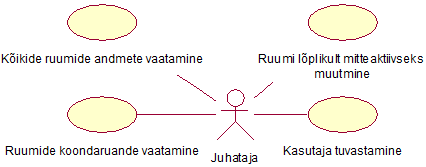
\includegraphics[width=0.8\textwidth]{./diagrams/sample-application-use-case-diagram.png}
\caption{Näidisrakenduse kasutusjuhtude diagramm.}
\label{fig_näidisrakendus_kasutusjuhtude_eskiismudel}
\end{figure}
\subsection{Kasutaja tuvastamine}
Kui kasutaja läheb lehele, mille nägemiseks peab ta olema autenditud, siis kuvatakse talle sisselogimise vorm, kuhu tuleb sisestada kasutajanimi ja parool (vt Joonis \ref{fig_näidisrakendus_kasutaja_tuvastamine}). Kui kasutajanimi ja parool on õiged, siis logitakse kasutaja sisse ning kasutaja näeb edaspidi autentimist nõudvate lehtede sisu.
\begin{figure}[H]
\centering
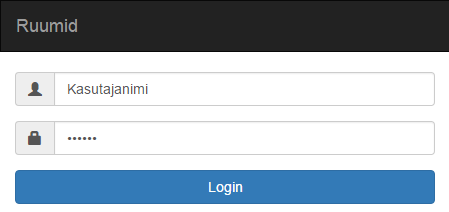
\includegraphics[width=0.8\textwidth]{./diagrams/sample-app-user-auth.png}
\caption{Näidisrakendus: Kasutaja tuvastamine.}
\label{fig_näidisrakendus_kasutaja_tuvastamine}
\end{figure}
\subsection{Ruumi lõplikult mitteaktiivseks muutmine}
Kasutajale kuvatakse vorm, kus kust ta saab valida millist ruumi ta muuta soovib (vt Joonis \ref{fig_näidisrakendus_vorm}). Ruumide loetelu saadakse vaate  \textit{public.active\_temporariliy\_inactive\_rooms} põhjal. Pärast vormi saatmist kutsutakse välja funktsioon \textit{functions.f\_permanently\_inactivate\_a\_room}. Kui funktsioon lõpetab oma töö ilma vigadeta, siis tagastatakse kasutajale teade, et vormi töötlemine õnnestus.
\begin{figure}[H]
\centering
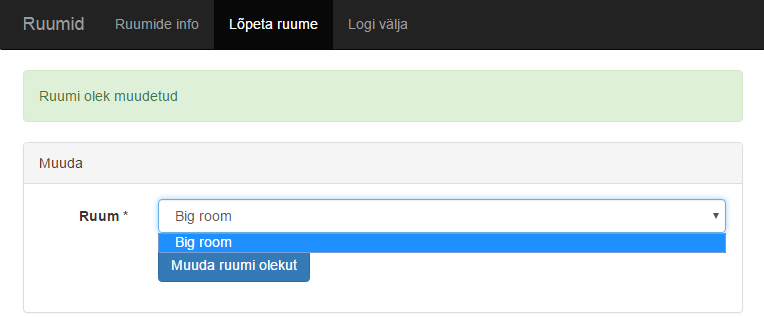
\includegraphics[width=\textwidth]{./diagrams/sample-app-form.png}
\caption{Näidisrakendus: Ruumi lõplikult mitteaktiivseks muutmine.}
\label{fig_näidisrakendus_vorm}
\end{figure}
\subsection{Ruumide koondaruande ja kõikide ruumide vaatamine}
Kasutajale kuvatakse ühel lehel nii ruumide koondaruanne kui ka kõikide ruumide info, kusjuures raportite read on võimalik jaotada mitmele leheküljele (vt Joonis \ref{fig_näidisrakendus_raportid})
\begin{figure}[H]
\centering
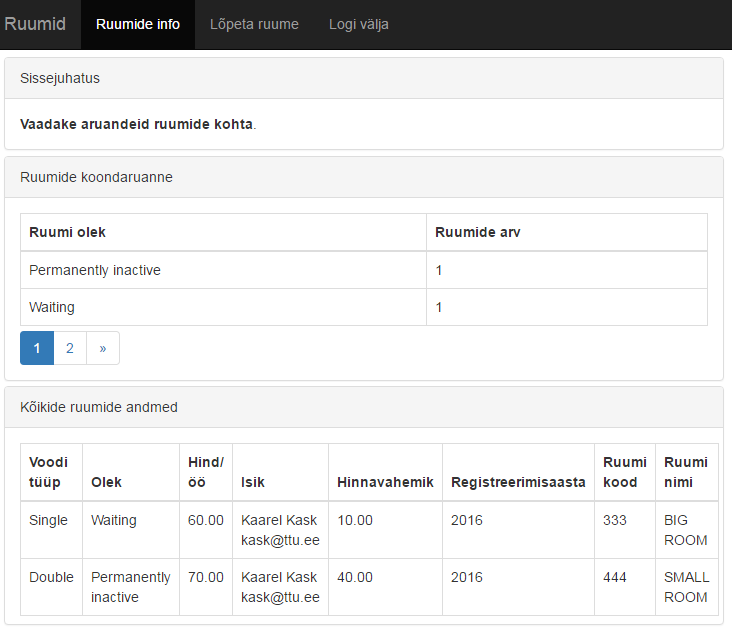
\includegraphics[width=\textwidth]{./diagrams/sample-app-reports.png}
\caption{Näidisrakendus: Ruumide koondaruande ja kõikide ruumide vaatamine.}
\label{fig_näidisrakendus_raportid}
\end{figure}

\section{Arendusvaade}
Loodud süsteemi funktsionaalsus on autori hinnangul piisav, et seda saaks reaalse tarkvara loomiseks kasutada, kuid edasiste iteratsioonide käigus võiks süsteemi kindlasti täiustada.
Kuna loodud süsteem võimaldab luua rakenduse ka metaandmete andmebaasile, siis saab süsteemi ennast kasutada süsteemi laienduste loomiseks.
Järgnevalt on esitatud loetelu funktsionaalsustest, mida võiks süsteemile lisada.
\begin{itemize}
\item Loodud rakenduse kirjeldust peaks olema võimalik eksportida ning importida. Sellisel juhul oleks võimalik rakendust varundada ning taastada ja kasutada versioonihaldustarkvara rakenduse versioonide haldamiseks. Kuna loodud süsteem kasutab ka ise andmebaasiliidest ning kõik rakendustega seotud tegevused tehakse läbi andmebaasifunktsioonide, siis saaks neid samu funktsioone kasutada rakenduste kirjeldamiseks. Sellisel juhul meenutaks loodud kirjeldus tavaprogrammeerimises tuttavaid funktsioonide väljakutseid, mis oleks semantiliselt arusaadavam kui tavaline andmetõmmis (\textit{data dump}).
\item Arendajal peaks olema võimalus näha vealogisid, sessiooniandmeid, vormidega saadetavaid andmeid ning muud abistavat infot, mis aitaksid probleemide korral rakendust siluda.
\item Loodud süsteem on hetkel ingliskeelne, et soodustada selle laiemat levikut. Arendajal võiks aga olla võimalus muuta kasutajaliideses kasutatavat keelt. Preagune tekst tuleb juba tõlkefailist ning seetõttu tuleks ainult realiseerida keelevaliku korral uute keelefailide sisselaadimine.
\item Hetkel saavad kõik rakendused kasutada üksnes eeldefineeritud malle. Iga rakenduse jaoks võiks aga saada luua spetsiifilisi malle, mis vastaksid täpselt rakenduse vajadustele.
\item Andmabaasiobjektid välistes andmebaasides võivad muutuda ning kaduda. Süsteem peaks olema võimeline kontrollima, millised andmebaasiobjektid on muutunud niivõrd, et ei võimalda rakendusel enam sihipäraselt töötada ning teavitada sellest arendajat.
\item Praeguses süsteemis sai realiseeritud neli erinevat regioonitüüpi: navigatsioon, HTML-tekst, raport ja vorm. Alati ei pruugi nendest aga piisata. Seetõttu tuleks uurida, millisel kujul oleks veel vaja infot kuvada ning realiseerida vastavad regioonid. Näiteks võiks olla võimalik kujutada infot graafikutena või punktidena maailmakaardil.
\item Arendajal oleks mugav rakendust arendada, kui ta saaks võimalikult palju tegevusi teha ühes ja samas keskkonnas. Seetõttu võiks süsteem võimaldada hallata välises andmebaasis olevaid andmebaasiobjekte ning andmeid.
\item Kui rakenduse kasutajad muudavad samal ajal samu andmeid, siis esimesena salvestatud andmed salvestatakse viimase poolt üle. Süsteem võiks sellisel juhul teavitada järgmist kasutajat, kes üritab salvestada, et andmed on vahepeal muutunud.
\item Süsteem võiks võimaldada luua REST-liideseid, mille abil saaksid nii loodavad rakendused, kui ka välised süsteemid välistest andmebaasidest infot küsida.
\item Realiseerida rakenduste loojatele väljapakkumiseks kasutajate autentimise meetod, mille korral igale rakenduse lõppkasutajale peab vastama andmebaasi kasutaja. See tähendab, et rakendusse logimisel tuleb sisestada andmebaasi kasutaja kasutajanimi ja parool ning lõppkasutaja saab teha andmebaasis (ja seega ka süsteemis) tegevusi andmebaasi kasutajale määratud õiguste piires.
\item Tulevikus peaks olema võimalik muuta rakenduse seisundit, mis omakorda määrab selle, kas see on kasutajatele kättesaadav või mitte. Praegu puudub võimalus rakenduse hetkeseisundi muutmiseks ja selle kaudu rakenduse lõppkasutajate eest peitmiseks. Hetkel on ainus võimalus rakendus kustutada. Arvestades ka sellega, et üksikut rakendust ei saa hetkel varundada ja taastada on see ebasoovitav variant.

\end{itemize}

%-------------------------------KOKKUVÕTE---------------------------
\section{Kokkuvõte}
Antud töö eesmärgiks oli luua PostgreSQL andmebaasisüsteemi põhine ja veebipõhine kiirprogrammeerimiskeskkond, mis võimaldaks luua veebirakendusi. Loodavad rakendused peavad suhtlema andmebaasiga läbi avaliku andmebaasiliidese ning rakenduste väljanägemist ning käitumist peab olema võimalik juhtida metaandmetega.\par

Töö käigus selgitati, kuidas seda eesmärki saavutada. Selleks oli vaja uurida, kuidas toimub andmete pärimine välisest andmebaasist ning kust saab infot andmebaasiobjektide kohta. Seejärel pandi paika esmased nõuded süsteemile, kirjeldati kasutusjuhud kõrgformaadis ning loodi olemi-suhte diagrammid, mis kirjeldasid süsteemi poolt vajatavaid metaandmeid.\par

Töö tulemusena valmis veebipõhine süsteem, mille loomiseks kasutati PHP-d, PostgreSQL-i, AngularJS-i, Bootstrapi ning Slim Framework-i. Süsteem võimaldab arendajatel luua veebirakendusi ning valida rakenduse autentimismeetodite vahel. Rakendusse saab luua lehti, mis omakorda sisaldavad regioone, mida antud töös realiseeriti neli erinevat tüüpi. HTML-regioon võimaldab lisada lehele HTML-vormindusega teksti. Navigatsiooni regiooni abil saab kuvada lehel navigeerimiseks vajaliku menüüd. Raportite regioon kuvab kasutajale vaate põhjal tabeli, mida on võimalik jagada mitmele leheküljele. Vormi regioon võimaldab küsida kasutajalt infot ning saata seda välisesse andmebaasi kutsudes välja välises andmebaasis oleva funktsiooni.\par

Loodud süsteem on arenduse esimese iteratsiooni tulemus ning seetõttu realiseeriti vaid oluliseimad funktsionaalsused, et tagada süsteemi esmane kasutatavus reaalse tarkvara loomiseks. Seetõttu esitati töös nägemus funktsionaalsustest, mida järgnevate iteratsioonide korral võiks süsteemile juurde lisada. Süsteemi lähtekoodi avaldamine võiks aidata kaasa sellele, et tulevikus selle arendamine jätkub.\par

Kõige olulisem põhimõtteline erinevus loodud arendussüsteemi ja Oracle APEX-i vahel seisneb selles, et Oracle APEX võimaldab luua rakenduse nii otse baastabelitele kui ka andmebaasi avalikule liidesele. Samas loodav süsteem nõuab, et rakendus kasutaks andmebaasi avaliku liidese elemente (vaated, materialiseeritud vaated, funktsioonid). Otse baastabelitele selle abil rakendusi luua ei saa ning tarkvara loomisel ei pakuta valikutesse baastabeleid.
\par
NuBuilder-ist, Xataface-st ja Mati Metsise magistritööst erineb loodud süsteem enim selle poolest, et loodud süsteemi puhul genereeritakse rakendused valmis andmebaasis, mitte rakenduskihis, kasutades võimalikult palju ära andmebaasi võimekust. Näiteks on töö tulemusena valminud süsteemis allsüsteemide teenindamiseks loodud 103 andmebaasis talletatud funktsiooni. Lisaks ei  nõua võrdluses välja toodud süsteemid andmebaasi avaliku liidese kasutamist.
\par
Mati Metsise magistritöö tulemusena valminud süsteemis loodi iga rakenduse jaoks samas andmebaasis uus skeem. Antud töö tulemusena valminud süsteem võimaldab aga luua rakendusi samas andmebaasiserveris olevate andmebaaside põhjal.
Lisaks võimaldavad antud töö tulemusena valminud süsteemi abil loodud rakendused teostada andmebaasides andmemuudatusi. Samuti realiseeriti suurem hulk erinevaid regiooni tüüpe.
\par

Loodud tulemuse valideerimiseks reliseeriti õppejõu poolt ette antud rakenduse kasutusjuhud, mis sarnanevad üliõpilastöödes esinevatele kasutusjuhtudele. Sellega sai süsteem edukalt hakkama ning seetõttu võib väita, et töö eesmärk saavutati. Näidisrakendus asub aadressil \url{http://apex.ttu.ee/pgapex/public/index.php/app/ruumid} (kasutajanimi: \textit{kask@ttu.ee}, parool: \textit{test}). Arenduskeskkond asub aadressil \url{http://apex.ttu.ee/pgapex}. \par

Töö tulemus on avaldatud MIT litsentsi all ning on avalikult kättesaadav aadressilt \newline \url{https://github.com/raitraidma/pgapex}.

\pagebreak

%------------------------------KASUTATUD KIRJANDUS-----------------------------------
\addcontentsline{toc}{section}{Kasutatud kirjandus}
\bibliographystyle{plain}
\bibliography{pgapex}

\pagebreak

%-----------------------------LISAD--------------------------------

\section*{Lisa 1 - PostgreSQL andmabaasisüsteemi süsteemikataloogid}
\label{lisa_postgresql_kataloogid}
\addcontentsline{toc}{section}{Lisa 1 - PostgreSQL andmabaasisüsteemi süsteemikataloogid}
\subsection*{information\_schema}
\begin{labeling}{element\_types}
\item [schemata] Sisaldab kõiki skeeme, millele kasutajal on ligipääs.
\item [views] Sisaldab kõiki vaateid, mis asuvad antud andmebaasis. Näidatakse ainult selliseid vaateid, millele kasutajal on ligipääs. Paraku ei saa sealt aga infot materialiseeritud vaadete kohta.
\item [columns] Sisaldab infot andmebaasis olevate tabelite ja vaadete veergude kohta. Näidatakse ainult neid veerge, millele kasutajal on ligipääs. Kui tagastatav tüüp on massiiv, siis saab selle kohta infot information\_schema.element\_types vaatest. Kui tagastatav tüüp on USER-DEFINED, siis saab selle kohta infot udt\_name veerust. Kui veerg on loodud domeeni põhjal, siis saab domeeni nime domain\_name veerust
\item [routines] Sisaldab infot andmebaasis olevate funktsioonide kohta, millele kasutajal on ligipääs. data\_type veerg sisaldab infot tagastatava tüübi kohta. Kui tagastatav tüüp on massiiv, siis saab selle kohta infot information\_schema.element\_types vaatest. Kui tagastatav tüüp on USER-DEFINED, siis saab selle kohta infot type\_udt\_name veerust.
\item [parameters] Sisaldab infot andmabaasis olevate funktsioonide parameetrite kohta. Parameetreid näidatakse ainult nende funktsioone kohta, millele kasutajal on ligipääs.
\item [element\_types] Sisaldab infot massiivi tüüpide kohta.
\end{labeling}
\cite{PostgreSQLInformationSchema}
\subsection*{pg\_catalog}
\begin{labeling}{pg\_namespace}
\item [pg\_database] Säilitab infot olemas olevate andmebaaside kohta. Erinevalt enamikest süsteemi kataloogidest on pg\_database jagatud kõikide klastrisse kuuluvate andmebaaside vahel.
\item [pg\_namespace] Säilitab infot nimeruumide kohta. Sealt on võimalik kätte saada andmebaasis olevad skeemid.
\item [pg\_shadow] Sisaldab infot kasutajate kohta, kellel on sisselogimisõigus. See tabel sisaldab paroole kujul 'md5' || md5(parool||kasutajanimi).
\item [pg\_class] Sisaldab infot kõige kohta, millel on veerud, või on mõnes muus mõttes tabeliga sarnane. Sealt saab infot vaadete ja materialiseeritud vaadete kohta. Selle tabeli pealt on tehtud ka vaates pg\_views ja pg\_matviews, millest on samuti võimalik küsida infot vastavalt vaadete ja materialiseeritud vaadete kohta. Lisaks ei pea kasutajatel olema reaalne ligipääs antud objektidele, et näha infot nende objektide kohta.
\item [pg\_attribute] Sisaldab infot veergude kohta.
\item [pg\_type] Sisaldab infot andmetüüpide kohta. Siin tabelis on esindatud nii põhiandmetüübid, kasutaja loodud tüübid, domeenid ja komposiitandmetüübid, mis luuakse iga andmebaasis oleva tabeli jaoks.
\item [pg\_proc] Sisaldab infot funktsioonide kohta.
\end{labeling}
\cite{PostgreSQLSystemCatalogs}

\section*{Lisa 2 - Free Software}
\label{lisa_free_software}
\addcontentsline{toc}{section}{Lisa 2 - Free Software}
\textit{Free Software} (Vaba tarkvara) tähendab, et kasutajatel on vabadus tarkvara käivitada, kopeerida, levitada, uurida, muuta ja täiustada. Seega \textit{Free Software} rõhub kasutaja vabadusele, mitte tarkvara hinnale. \par
Tarkvara on \textit{Free Software}, kui selle kasutajate jaoks on täidetud neli olulist kriteeriumit:
\begin{itemize}
\item Vabadus 0: käivitada programmi oma suva järgi, ükskõik mis eesmärgil
\item Vabadus 1: uurida, kuidas programm töötab ja seda muuta (eeldab ligipääsu lähtekoodile)
\item Vabadus 2: levitada antud tarkvara
\item Vabadus 3: levitada antud tarkvara muudetud kujul (eeldab ligipääsu lähtekoodile)
\end{itemize}
Vabadus levitada (vabadused 2 ja 3) tähendab vabadust jagada antud tarkvara muudetud või muutmata kujul kas tasu eest või tasuta - selleks ei pea kelleltki luba küsima. Küll aga peab jagatav koopia sisaldama nii lähtekoodi kui ka käivitatavat programmi (kui programmeerimiskeel toetab seda võimalust)\par
\textit{Free Software} ei tähenda, et tegu ei võiks olla kommertstarkvaraga. \textit{Free Software} võib omandada tasuta või raha eest. Vaatamata sellele, kuidas koopia antud tarkvarast omandati,  jääb omandajale vabadus antud tarkvara jagada, muuta ja müüa.
\cite{GNU_Free_SW}

\section*{Lisa 3 - Open Source}
\label{lisa_open_source}
\addcontentsline{toc}{section}{Lisa 3 - Open Source}
\textit{Open Source} (Avatud lähtekood) ei tähanda ainult ligipääsu lähtekoodile. Tarkvara levitamisel peab lähtuma järgmistest reeglitest:
\begin{enumerate}
\item Vaba jagamine - Litsents ei tohi piirata ühtegi osapoolt tarkvara müümast või jagamast.
\item Lähtekood -  Tarkvara peab sisaldama lähtekoodi ning lähtekoodi ja kompileeritud koodi jagamine peab olema lubatud. Kui tarkvara ei jagata koos lähtekoodiga, peab lähtekood olema mujalt mõistliku vaevaga kättesaadav.
\item Tuletatud tarkvara - Litsents peab lubama muudatusi ja tuletatud tarkvara ning peab lubama nende jagamist samadel litsentsitingimustel.
\item Autori lähtekoodi terviklikkus - Litsents võib keelata muudetud lähtekoodi jagamist üksnes siis, kui on lubatud jagada paikefaile (\textit{patch file}), et muuta programmi lähtekoodi selle loomise mingis järgus (\textit{build time}). Litsents peab selgelt lubama muudetud lähtekoodiga tarkvara jagamist. Litsents võib nõuda, et tuletatud tarkvara kannaksid teist nime või versiooninumbrit, kui originaaltarkvara.
\item Isikute või gruppide diskrimineerimiskeeld - Litsents ei tohi diskrimineerida ühtegi isikut või isikute gruppi.
\item Tegevusvaldkonna diskrimineerimiskeeld - Litsents ei tohi piirata ühtegi konktreetset tegevusvaldkonda.
\item Litsentsi jagamine - Programmile sätestatud õigused kehtivad kõigile, kellele programm on jagatud, ilma, et osapooled vajaksid täiendavat litsentsi.
\item Litsents ei tohi olla tootespetsiifiline - Programile sätestatud õigused ei tohi sõltuda sellest, kas programm kuulub mõne teise programmi koosseisu.
\item Litsents ei tohi piirata teisi tarkvarasid - Litsents ei tohi panna piiranguid teistele tarkvaradele, mida jagatakse koos antud tarkvaraga.
\item Litsents peab olema tehnoloogiliselt neutraalne - Ükski klausel ei tohi viidata konkreetsele tehnoloogiale, stiilile või liidesele.
\end{enumerate}
\cite{Open_Source_Def}

\section*{Lisa 4 - Populaarsemate litsentside võrdlus}
\label{lisa1}
\addcontentsline{toc}{section}{Lisa 4 - Populaarsemate litsentside võrdlus}
\begin{table}[H]
\centering
\caption{Populaarsemate litsentside võrdlus.}
\label{table_litsentside_vordlus}
\begin{tabular}{|p{3cm}|p{4cm}|p{4cm}|p{4cm}|}
\hline
\rowcolor{rowgray}
 & Nõutud & Lubatud & Keelatud \\ \hline
MIT & Litsents ja copyright märge & Kaubanduslik kasutamine & Võtta vastutusele \\
 &  & Jagamine &  \\
 &  & Muutmine &  \\
 &  & Privaatne kasutamine &  \\ \hline
Apache \newline License 2.0 & Litsents ja copyright märge & Kaubanduslik kasutamine & Võtta vastutusele \\
 & Teavitus muudatustest & Jagamine & Kasutada kaubamärki \\
 &  & Muutmine &  \\
 &  & Patendi kasutamine &  \\
 &  & Privaatne kasutamine &  \\ \hline
GNU GPLv3 & Lähtekoodi avaldamine & Kaubanduslik kasutamine & Võtta vastutusele \\
GNU GPLv2 & Litsents ja copyright märge & Jagamine &  \\
 & Sama litsents & Muutmine &  \\
 & Teavitus muudatustest & Patendi kasutamine &  \\
 &  & Privaatne kasutamine & \\ \hline
\end{tabular}
\cite{Licences}
\end{table}
\pagebreak

\section*{Lisa 5 - Kasutusjuhtude diagrammid}
\addcontentsline{toc}{section}{Lisa 5 - Kasutusjuhtude diagrammid}
Alljärgnevalt on esitatud kasutusjuhtude diagrammid allsüsteemide kaupa.

\subsection*{Rakenduste funktsionaalne allsüsteem}
\begin{figure}[H]
\centering
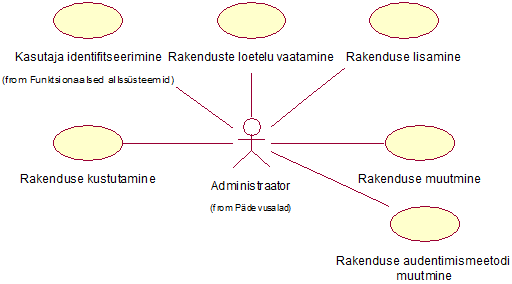
\includegraphics[width=\textwidth]{./diagrams/applications-subsystem-use-case-digram.png}
\caption{Rakenduste funktsionaalse allsüsteemi kasutusjuhtude diagramm.}
\label{fig_rakenduste_funktsionaalse_allsüsteemi_kasutusjuhtude_eskiismudel}
\end{figure}

\subsection*{Lehtede funktsionaalne allsüsteem}
\begin{figure}[H]
\centering
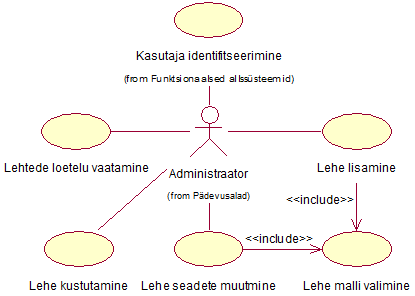
\includegraphics[width=0.8\textwidth]{./diagrams/pages-subsystem-use-case-digram.png}
\caption{Lehtede funktsionaalse allsüsteemi kasutusjuhtude diagramm.}
\label{fig_lehtede_funktsionaalse_allsüsteemi_kasutusjuhtude_eskiismudel}
\end{figure}

\subsection*{Regioonide funktsionaalne allsüsteem}
\begin{figure}[H]
\centering
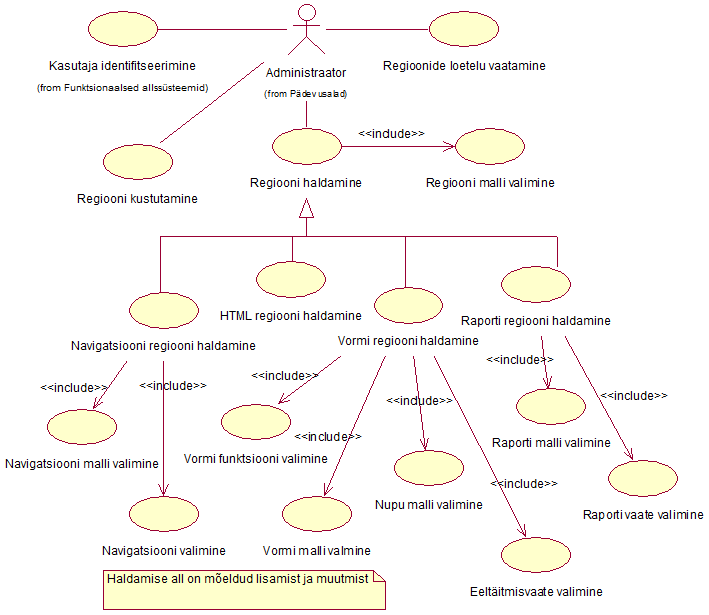
\includegraphics[width=\textwidth]{./diagrams/regions-subsystem-use-case-digram.png}
\caption{Regioonide funktsionaalse allsüsteemi kasutusjuhtude diagramm.}
\label{fig_regioonide_funktsionaalse_allsüsteemi_kasutusjuhtude_eskiismudel}
\end{figure}

\subsection*{Navigatsioonide funktsionaalne allsüsteem}
\begin{figure}[H]
\centering
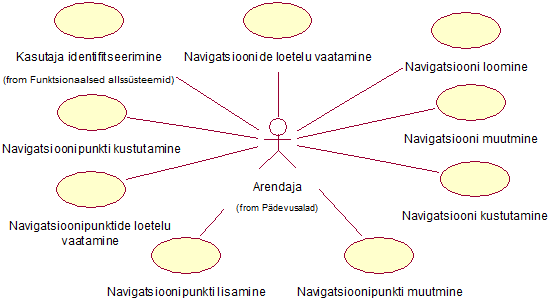
\includegraphics[width=\textwidth]{./diagrams/navigations-subsystem-use-case-digram.png}
\caption{Navigatsioonide funktsionaalse allsüsteemi kasutusjuhtude diagramm.}
\label{fig_navigatsioonide_funktsionaalse_allsüsteemi_kasutusjuhtude_eskiismudel}
\end{figure}

\pagebreak

\section*{Lisa 6 - Andmebaasi diagrammid}
\label{lisa_andmebaasi_diagrammid}
\addcontentsline{toc}{section}{Lisa 6 - Andmebaasi diagrammid}
Järgnevalt on välja toodud andmebaasidiagrammid registrite kaupa.

\subsection*{Andmebaasiobjektide register}
Andmebaasiobjekte kirjeldavad tabelid realiseeriti materialiseeritud vaadetena. Kuna vaadetes olevaid veerge ei saa kasutada välisvõtmekitsendustes, siis sisaldavad alltoodud vaated rohkem infot kui olemi-suhte diagrammidel näha. Sedasi tagatakse iga rea unikaalsus.\par
Arenduskeskkonna kasutajale on loodud nupp, millele vajutades tema loodava rakenduse andmebaasi kirjeldust värskendatakse.
\begin{figure}[H]
\centering
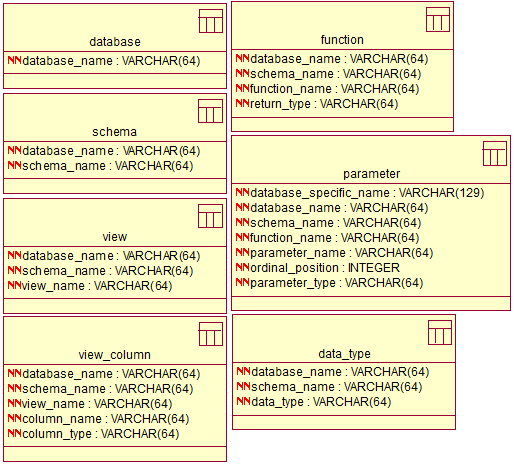
\includegraphics[width=0.8\textwidth]{./diagrams/database-object-db-diagram.png}
\caption{Andmebaasiobjektide registri andmebaasi diagramm.}
\label{fig_andmebaasiobjektide_registri_andmebaasi_diagramm}
\end{figure}

\subsection*{Rakenduste register}
\begin{figure}[H]
\centering
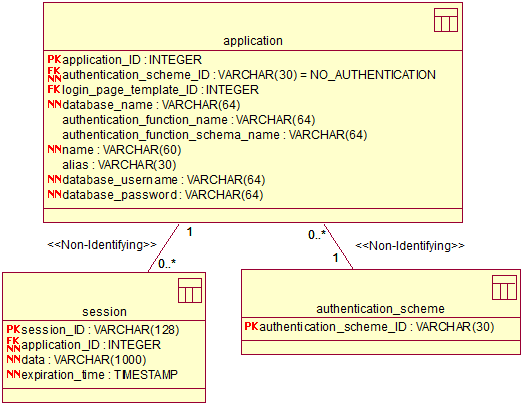
\includegraphics[width=0.9\textwidth]{./diagrams/applications-db-diagram.png}
\caption{Rakenduste registri andmebaasi diagramm.}
\label{fig_rakenduste_registri_andmebaasi_diagramm}
\end{figure}

\subsection*{Lehtede register}
\begin{figure}[H]
\centering
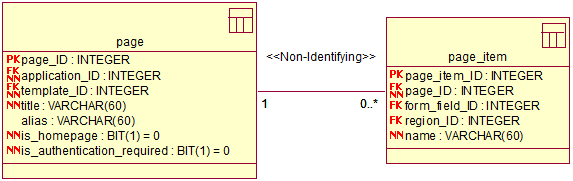
\includegraphics[width=0.9\textwidth]{./diagrams/page-db-diagram.png}
\caption{Lehtede registri andmebaasi diagramm.}
\label{fig_lehtede_registri_andmebaasi_diagramm}
\end{figure}

\subsection*{Regioonide register}
\begin{figure}[H]
\centering
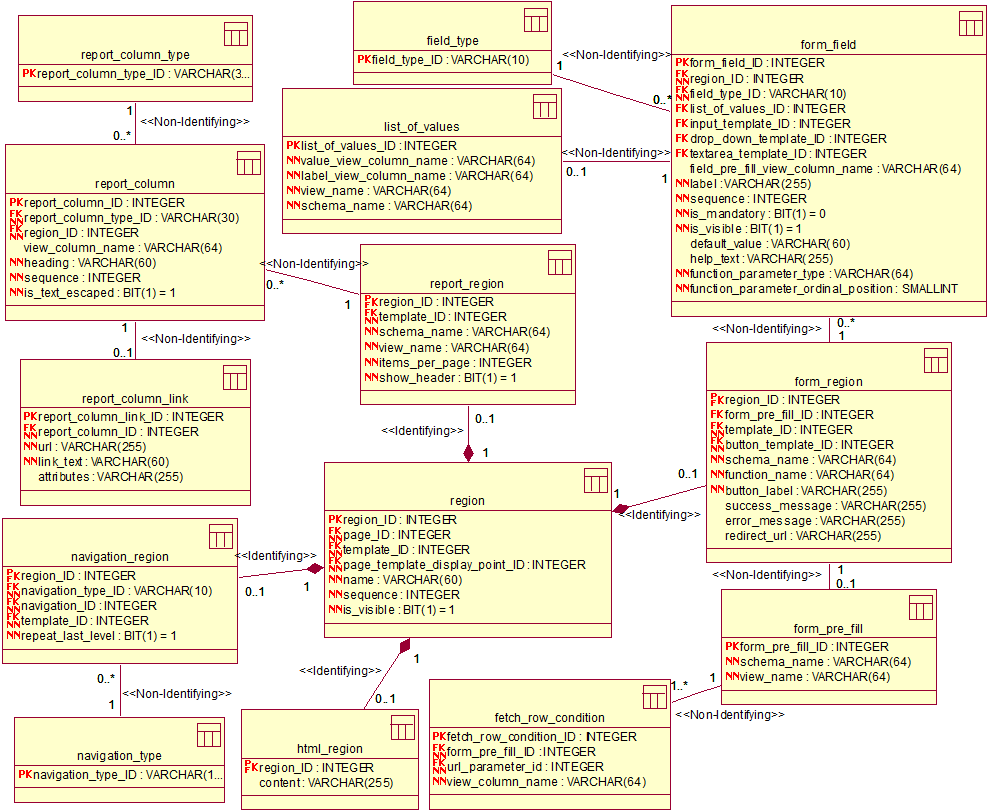
\includegraphics[width=\textwidth]{./diagrams/region-db-diagram.png}
\caption{Regioonide registri andmebaasi diagramm.}
\label{fig_regioonide_registri_andmebaasi_diagramm}
\end{figure}

\subsection*{Navigatsioonide register}
\begin{figure}[H]
\centering
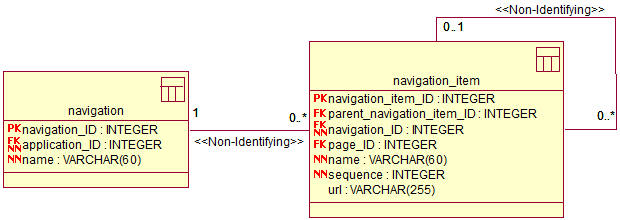
\includegraphics[width=\textwidth]{./diagrams/navigation-db-diagram.png}
\caption{Navigatsioonide registri andmebaasi diagramm.}
\label{fig_navigatsioonide_registri_andmebaasi_diagramm}
\end{figure}

\subsection*{Mallide register}
\begin{figure}[H]
\centering
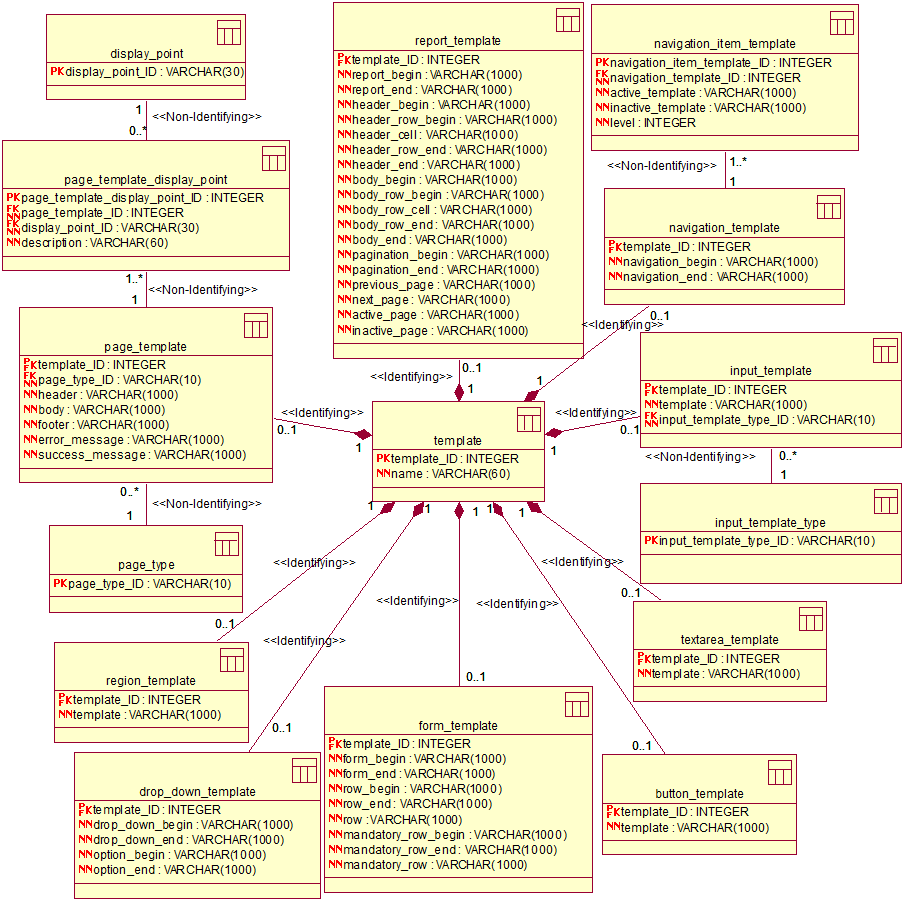
\includegraphics[width=\textwidth]{./diagrams/template-db-diagram.png}
\caption{Mallide registri andmebaasi diagramm.}
\label{fig_mallide_registri_andmebaasi_diagramm}
\end{figure}

\pagebreak

\section*{Lisa 7 - Ekraanipildid loodud arenduskeskkonnast}
\label{lisa_kasutajaliidese_ekraanipildid}
\addcontentsline{toc}{section}{Lisa 7 - Kasutajaliidese ekraanipildid}
Järgnevalt on välja toodud väike osa süsteemi kuvadest, et anda lugejale aimdus sellest, milline süsteem välja näeb.
Selleks, et ekraanipildid lehtedele ära mahuksid, on mõningatel piltidel vormielementide laiusi ning nende vahelisi kaugusi vähendatud.

\begin{figure}[H]
\centering
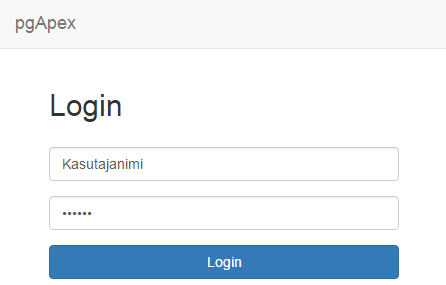
\includegraphics[width=0.6\textwidth]{./diagrams/pgapex-login.png}
\caption{Loodud süsteem: Autentimine.}
\label{fig_loodud_süsteem_autentimine}
\end{figure}

\begin{figure}[H]
\centering
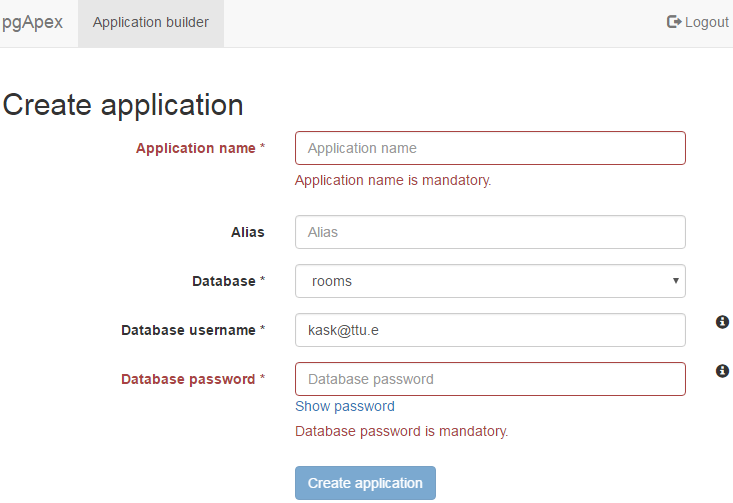
\includegraphics[width=\textwidth]{./diagrams/pgapex-create-application.png}
\caption{Loodud süsteem: Rakenduse loomine.}
\label{fig_loodud_süsteem_rakenduse_loomine}
\end{figure}
\pagebreak

Selleks et raportis loodud link suunaks näiteks samas rakenduses lehele, mille alias on ``muuda'', ning annaks URL-parameetrile \textit{p\_room\_code\_old} kaasa vaate veerus \textit{room\_code} oleva väärtuse, tuleb URL-aadressi välja lisada järgnev tekst:\newline \&APPLICATION\_ROOT\&/app/\&APPLICATION\_ID\&/muuda?p\_room\_code\_old=\%room\_code\%.
\begin{figure}[H]
\centering
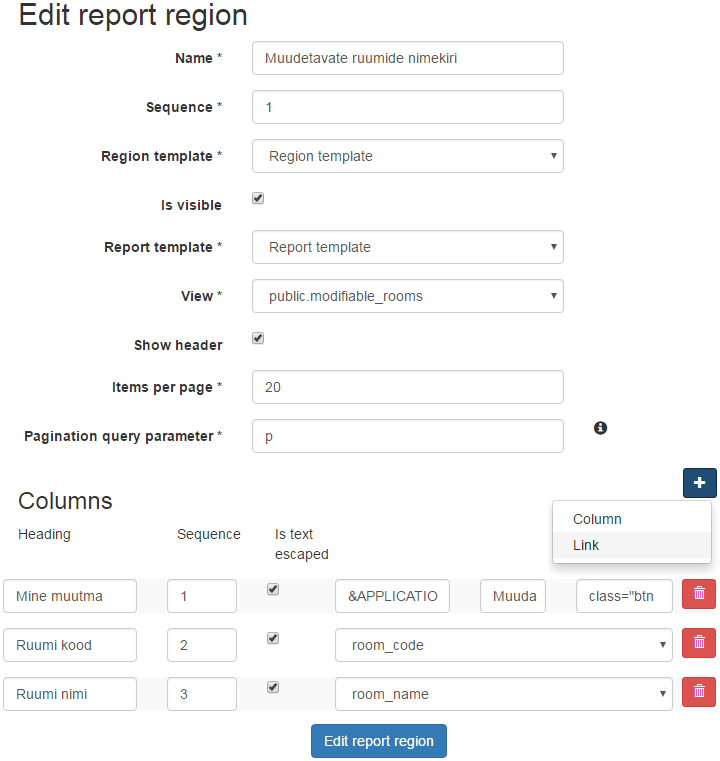
\includegraphics[width=\textwidth]{./diagrams/pgapex-edit-report-region.png}
\caption{Loodud süsteem: Raporti regiooni muutmine.}
\label{fig_loodud_süsteem_raporti_regiooni_muutmine}
\end{figure}

\begin{figure}[H]
\centering
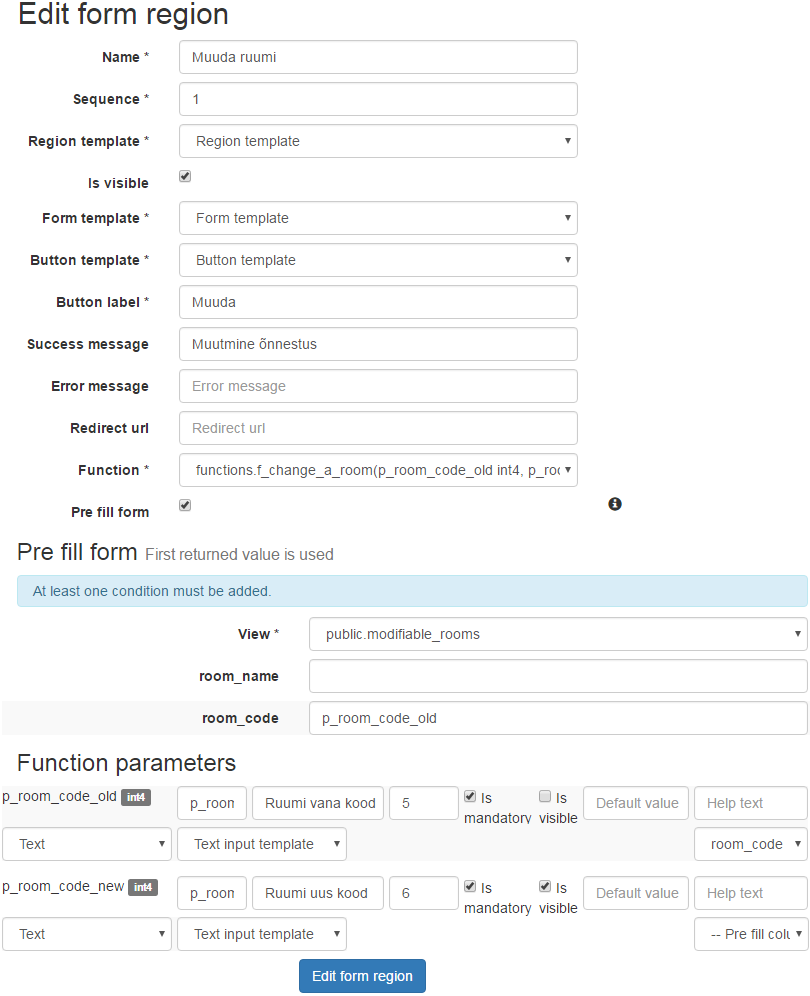
\includegraphics[width=\textwidth]{./diagrams/pgapex-edit-form-region.png}
\caption{Loodud süsteem: Vormi regiooni muutmine.}
\label{fig_loodud_süsteem_vormi_regiooni_muutmine}
\end{figure}

\section*{Lisa 8 - Andmebaasiobjektide info küsimine PostgreSQL andmebaasisüsteemis}
\addcontentsline{toc}{section}{Lisa 8 - Metaandmete küsimine PostgreSQL andmebaasisüsteemis}
Järgnevalt on esitatud mõned päringud, millega küsitakse infot andmebaasis olevate andmebaasiobjektide kohta.
\par
Kuna \textit{information\_schema} ei sisalda infot materialiseeritud vaadete kohta, siis küsitakse seda infot \textit{pg\_catalog}-st (vt Joonis \ref{sql_vaadete_metainfo_küsimine}).
\begin{figure}[H]
\centering
\begin{SQL}
SELECT n.nspname AS view_schema, c.relname AS view_name
FROM pg_catalog.pg_class c
LEFT JOIN pg_catalog.pg_namespace n ON n.oid = c.relnamespace
WHERE c.relkind IN ('v', 'm')
  AND n.nspname NOT IN ('information_schema', 'pg_catalog')
  AND n.nspname NOT LIKE 'pg_toast%'
  AND n.nspname NOT LIKE 'pg_temp%'
\end{SQL}
\caption{SQL: Andmebaasis vastavas skeemis olevate vaadete ja materialiseeritud vaadete küsimine.}
\label{sql_vaadete_metainfo_küsimine}
\end{figure}

Kuna ühes skeemis võib olla mitu sama nimega funktsiooni, siis nende unikaalsuse tagamiseks on võetud kasutusele väli \textit{specific\_name} (vt Joonis \ref{sql_funktsiooni_parameetrite_metainfo_küsimine}).

\begin{figure}[H]
\centering
\begin{SQL}
SELECT r.specific_name, r.routine_schema, r.routine_name, p.parameter_name, p.ordinal_position, p.udt_name
FROM information_schema.routines r
JOIN information_schema.parameters p ON r.specific_name = p.specific_name
WHERE r.routine_type = 'FUNCTION'
  AND r.routine_schema NOT IN ('pg_catalog', 'information_schema')
\end{SQL}
\caption{SQL: Andmebaasis vastavas skeemis oleva funktsiooni parameetite info küsimine.}
\label{sql_funktsiooni_parameetrite_metainfo_küsimine}
\end{figure}

\end{document}
